\documentclass[11pt,a4paper]{article}
\usepackage[T1]{fontenc}
\usepackage[british]{babel}
\usepackage{amsmath,amssymb,amsthm}
\usepackage{booktabs,array,longtable}
\usepackage[margin=22mm]{geometry}
\usepackage{pgfplots}
\definecolor{plotgreen}{HTML}{279E68}
\definecolor{panelblue}{HTML}{1F77B4}
\definecolor{panelcyan}{HTML}{17BECF}
\definecolor{plotblue}{HTML}{256C88}
\definecolor{plotslate}{HTML}{7B8DA2}
\definecolor{plotink}{HTML}{17384F}
\pgfplotsset{compat=1.18}
\usepackage[hidelinks]{hyperref}
\newcommand{\E}{\mathbb E}
\newcommand{\Pp}{\mathbb P}
\newcommand{\Q}{\mathbb Q}
\newcommand{\F}{\mathcal F}
\newcommand{\ind}{\mathbf 1}
\newcommand{\CVaR}{\operatorname{CVaR}}
\newcommand{\VaR}{\operatorname{VaR}}
\newcommand{\SE}{\operatorname{SE}}
\newcommand{\Var}{\operatorname{Var}}
\newcommand{\Cov}{\operatorname{Cov}}
\newcommand{\IF}{\operatorname{IF}}
\newcommand{\sd}{\operatorname{sd}}
\newcommand{\relu}{\operatorname{ReLU}}
\newcommand{\dt}{\Delta t}
\newtheorem{proposition}{Proposition}
\newtheorem{lemma}{Lemma}
\theoremstyle{remark}
\newtheorem*{remark}{Remark}
\setlength{\parindent}{1.2em}
\setlength{\parskip}{2pt}
\setlength{\emergencystretch}{2em}
\renewcommand{\arraystretch}{1.15}
\hypersetup{pdftitle={An independent numerical reconstruction of the deep-hedging experiment},pdfauthor={Amanjeet Singh}}
\title{An independent numerical reconstruction\\of the deep-hedging experiment}
\author{Amanjeet Singh}
\date{8 October 2026}
\begin{document}
\maketitle
\vspace{-1.5em}
\section{Scope, notation and contract}
I study the 95\% CVaR hedge for a 63-day European call under the paper's GJR--GARCH dynamics. I compare its hedging loss and the deep-minus-delta strategy with the published 95\% results, then extend the comparison to the 85\% and 90\% agents in Figure~1, Panel~B. I also examine the standalone hedging-profit distributions and their sample centres.

Dates are $t=0,\ldots,T$, with $T=63$ and $\dt=1/252$ years. The stock price and strike are $S_0=K=100$, the continuously compounded annual risk-free rate is $r=0.0167$, and the dividend yield is $q=0.0165$. Write $c=(r-q)\dt$. The terminal call payoff is $H=(S_T-K)^+$. Both base hedges start with capital $V_0=3.16$, as reported in the paper, and incur no transaction costs. The neural strategy may borrow at most $B=100$ units of cash. Positions are chosen using information available at the decision date.

The symbol $h_t$ denotes the conditional variance known at date $t$ for the next log return $R_{t+1}$. Thus $h_t$ corresponds to $\sigma_{t+1}^2$ in the paper's state convention. The GJR coefficient is $\alpha$; the risk-confidence level is separately denoted $a=0.95$. Probability measures $\Pp$, $\Q$ and $\Q^S$ denote the physical, selected pricing and total-return-stock measures. Hedge wealth, shares and cash are $V_t$, $\delta_t$ and $\phi_t=V_t-\delta_tS_t$. The conditional option delta is $\Delta_t$; $U_t$ is the wealth of the zero-capital deep-minus-delta strategy. Positive hedging loss $L=H-V_T$ means a short-call funding shortfall. All monetary results use the normalised initial index level 100.

Write $\varphi(z)=e^{-z^2/2}/\sqrt{2\pi}$ and $\Phi(b)=\int_{-\infty}^b\varphi(z)\,dz$ for the standard normal density and distribution function.
The filtration $\F_t$ contains the initial state and market innovations through date $t$; with policy parameters fixed, hedge positions and wealth are adapted to it.

\section{Historical data and calibration}
\subsection{Return sample and likelihood}
The public data file \texttt{SP500\_random.csv} contains 6,291 closing observations. The slice beginning at zero-based row 5,031 starts on 31 December 2015, which supplies the preceding close for the first return on 4 January 2016. The final return is 31 December 2020. There are $n_{\mathrm{hist}}=1,259$ log returns
\begin{equation}
\begin{aligned}
 r_i&=\log\frac{\mathrm{Close}_i}{\mathrm{Close}_{i-1}},\qquad u_i=r_i-\mu,\\
 v_{i+1}&=\omega+(\alpha+\gamma\ind_{\{u_i<0\}})u_i^2+\beta v_i.
\end{aligned}
 \label{eq:likelihoodstate}
\end{equation}
Here $v_i$ is the conditional variance of return $r_i$. The daily sample mean is $0.0004833152718719082$. The sample standard deviation, using denominator $n_{\mathrm{hist}}-1$, is $0.01218067623362892$. Multiplication by $\sqrt{252}$ gives the annualised value $0.193362240688662$.

Under the conditional Gaussian assumption,
\begin{equation}
 f(r_i\mid\F_{i-1})=\frac{1}{\sqrt{2\pi v_i}}
       \exp\!\left(-\frac{u_i^2}{2v_i}\right).
\end{equation}
Multiplication of these conditional densities and taking logarithms gives
\begin{equation}
 \ell(\mu,\omega,\alpha,\gamma,\beta)
 =-\frac12\sum_{i=1}^{1,259}
       \left[\log(2\pi)+\log v_i+\frac{u_i^2}{v_i}\right].
 \label{eq:likelihood}
\end{equation}
I fit the constant-mean Gaussian model using
\begin{verbatim}
arch_model(returns, vol="Garch", p=1, o=1, q=1,
           rescale=False).fit(disp="off")
\end{verbatim} ARCH~8.0.0 initialises the likelihood variance with a backcast of preliminary squared residuals: $\sum_{j=0}^{m-1}w_ju_j^2$, where $m=\min(75,n_{\mathrm{hist}})$, $w_j=0.94^j/\sum_{k=0}^{m-1}0.94^k$. Its constrained SLSQP fit imposes $\omega\geq0$, $\alpha\geq0$, $\beta\geq0$, $\alpha+\gamma\geq0$ and $\alpha+\gamma/2+\beta\leq1$, with a strictly positive numerical lower bound for $\omega$ and the library's likelihood variance safeguards. These fitting safeguards do not define the simulation's initial variance.

\begin{table}[htbp]
\centering
\small
\caption{Full-precision retained parameters and conditioning control, in decimal-return units. The control is not used for training.}
\label{tab:parameters}
\begin{tabular}{@{}lll@{}}
\toprule
Parameter & Retained source-method fit & Scaled conditioning control\\
\midrule
$\mu$ & $0.0006252906867408154$ & $0.0006821386109908009$ \\
$\omega$ & $2.965710904850983\times 10^{-6}$ & $3.840432081072945\times 10^{-6}$ \\
$\alpha$ & $0.1000004458628082$ & $0.147309671265852$ \\
$\gamma$ & $0.1999994343814858$ & $0.2306995641759462$ \\
$\beta$ & $0.7799996137183315$ & $0.7207770282209127$ \\
$h_0$ & $2.608312112499664\times 10^{-5}$ & $2.566290077158296\times 10^{-5}$ \\
\bottomrule
\end{tabular}
\end{table}

\subsection{Scaling and initial-state ambiguity}
I apply the source procedure directly to decimal returns. The retained fit reports convergence flag zero after eight optimisation iterations and log likelihood $4298.041204605$. For the conditioning control, I fit $100r_i$, then divide the mean by 100 and the variance intercept by $100^2$; $\alpha$, $\gamma$ and $\beta$ are unchanged by unit conversion. For $Y=100R$, the density transformation is $f_Y(y)=f_R(y/100)/100$. Consequently,
\begin{equation}
 \ell_{\rm decimal}=\ell_{\rm percentage}+1,259\log100
 =-1497.119726825+1,259\log100=4300.789537334.
 \label{eq:scaling}
\end{equation}
The control converges after twelve iterations and has a larger comparable likelihood. A success flag therefore does not establish that the unscaled fit is the global maximum. I retain the unscaled source-method result for this experiment without replacing it after inspection of test results.

I use the retained terminal fitted variance in Table~\ref{tab:parameters} as the known first-return variance $h_0$. Updating it with the final observed residual would instead give $2.666633546772747\times 10^{-5}$; the analogous forecast from the scaling control is $2.718451102985524\times 10^{-5}$. This choice fixes the initial state of the experiment; the published simulation's initial variance is unspecified. The paper's printed $\alpha=0.11$ also differs from the source-method fit near 0.10, and the printed $\omega=0.01\%$ does not specify enough units to reconstruct the daily-variance intercept.

\section{Physical dynamics and the selected pricing measure}
\subsection{Physical simulation}
Under $\Pp$, independently sampled innovations $\varepsilon_{t+1}\sim N(0,1)$ give
\begin{align}
 R_{t+1}&=\mu+\sqrt{h_t}\,\varepsilon_{t+1}, &
 S_{t+1}&=S_t\exp(R_{t+1}),\label{eq:physicalstock}\\
 h_{t+1}&=\omega+h_t(\alpha+\gamma\ind_{\{\varepsilon_{t+1}<0\}})
                           \varepsilon_{t+1}^2+\beta h_t.
 \label{eq:physicalvariance}
\end{align}
At each date, I store the known state, draw the return innovation, advance the stock, and then update the variance. No artificial initial innovation precedes the first return. This order supplies the policy with the variance of its next return.

I generate 400,000 training paths with seed~43, 50,000 validation paths with seed~44, and 100,000 test paths with seed~45 using three independent \texttt{NumPy RandomState} streams. Each path contains 63 decisions and 63 innovations. I compute the stock and variance recursion in float64, then convert the stored log spots, one-period gains, annualised next-return volatilities and terminal payoffs to float32 for network computation. The transformation $\sqrt{252h_t}$ is a fixed feature scaling.

\subsection{Conditional density change}
For a standard normal variable $Z$ and any finite real $a$, completion of the square gives
\begin{align}
 \E[e^{aZ}]&=\frac1{\sqrt{2\pi}}
       \int_{\mathbb R}\exp(az-z^2/2)\,dz\nonumber\\
 &=e^{a^2/2}\frac1{\sqrt{2\pi}}
       \int_{\mathbb R}\exp[-(z-a)^2/2]\,dz
 =e^{a^2/2}.
 \label{eq:normalmgfsteps}
\end{align}
Consequently a conditionally Gaussian log return of mean $m_t$ and variance $h_t$ satisfies
\begin{equation}
 \E[e^{R_{t+1}}\mid\F_t]=e^{m_t+h_t/2}.
\end{equation}
The pricing condition is $\E_{\Q}[e^{R_{t+1}}\mid\F_t]=e^c$, where $c=(r-q)\dt$. Taking logarithms shows that $m_t=c-h_t/2$. The physical log-return mean is $\mu$, so the predictable shift required to obtain this mean is
\begin{equation}
 \eta_t=\frac{\mu-c+h_t/2}{\sqrt{h_t}},\qquad
 \Lambda_{t+1}=\exp\!\left(-\eta_t\varepsilon_{t+1}
                                    -\frac{\eta_t^2}{2}\right).
 \label{eq:measurechange}
\end{equation}
Here $h_t>0$ is known at date $t$. For the reported coefficients, all finite-horizon variance states are finite and positive almost surely: the variance update is finite for finite innovations and is bounded below by $\omega>0$. The coefficients satisfy $\alpha\geq0$, $\alpha+\gamma\geq0$ and $\beta\geq0$.

Using \eqref{eq:normalmgfsteps} conditionally,
\begin{equation}
 \E_{\Pp}[\Lambda_{t+1}\mid\F_t]
 =e^{-\eta_t^2/2}\E_{\Pp}[e^{-\eta_t\varepsilon_{t+1}}\mid\F_t]
 =e^{-\eta_t^2/2}e^{\eta_t^2/2}=1.
\end{equation}
Set $L_0^{\Q}=1$ and $L_t^{\Q}=\prod_{j=1}^t\Lambda_j$. Then
\begin{equation}
 \E_{\Pp}[L_{t+1}^{\Q}\mid\F_t]
 =L_t^{\Q}\E_{\Pp}[\Lambda_{t+1}\mid\F_t]=L_t^{\Q}.
\end{equation}
Induction gives $\E_{\Pp}[L_t^{\Q}]=1$. Thus the positive process defines a probability measure on the finite horizon by $d\Q/d\Pp=L_T^{\Q}$. Its one-step conditional density is obtained by multiplying the physical normal density by $\Lambda_{t+1}$:
\begin{align}
 \varphi(e)\exp(-\eta_te-\eta_t^2/2)
 &=\frac1{\sqrt{2\pi}}
      \exp[-e^2/2-\eta_te-\eta_t^2/2]\nonumber\\
 &=\frac1{\sqrt{2\pi}}\exp[-(e+\eta_t)^2/2].
\end{align}
Therefore $Z_{t+1}=\varepsilon_{t+1}+\eta_t$ is standard normal conditionally on $\F_t$ under $\Q$. Its conditional law does not depend on the past. Iterating these conditional laws justifies drawing successive independent standard $\Q$ normals.

Substitution into the physical return gives
\begin{align}
 R_{t+1}
 &=\mu+\sqrt{h_t}(Z_{t+1}-\eta_t)\nonumber\\
 &=\mu-(\mu-c+h_t/2)+\sqrt{h_t}Z_{t+1}
 =c-h_t/2+\sqrt{h_t}Z_{t+1}.
 \label{eq:qstock}
\end{align}
The variance is the same pathwise function of the physical innovation, so the substitution must also be made there:
\begin{equation}
 h_{t+1}=\omega+h_t[\alpha+\gamma\ind_{\{Z_{t+1}-\eta_t<0\}}]
                  (Z_{t+1}-\eta_t)^2+\beta h_t.
 \label{eq:qvariance}
\end{equation}
Using $Z_{t+1}$ without the shift in \eqref{eq:qvariance} would produce a different model. Finally,
\begin{align}
 \E_{\Q}[S_{t+1}\mid\F_t]
 &=S_te^{c-h_t/2}\E_{\Q}[e^{\sqrt{h_t}Z_{t+1}}\mid\F_t]\nonumber\\
 &=S_te^{c-h_t/2}e^{h_t/2}=S_te^c.
\end{align}
Starting from finite $S_0$, non-negativity and repeated conditional expectation give $\E_{\Q}[S_t]=S_0e^{ct}<\infty$. Hence $e^{-ct}S_t$ is a true finite-horizon $\Q$ martingale, and more generally
\begin{equation}
 \E_{\Q}[S_{t+\tau}\mid\F_t]=S_te^{c\tau}.
 \label{eq:qfirstmomentsteps}
\end{equation}
I implement the particular measure specified in the paper's footnote~3 through this construction. It does not assert uniqueness of the pricing measure in an incomplete market.

\section{Initial price and the missing initial state}
\subsection{Final-period integration}
The call price under the selected measure is $C_0=e^{-rT\dt}\E_{\Q}[(S_T-K)^+]$. I estimate it through a bounded put, avoiding an assumption that direct call-payoff observations have finite variance. For a final-period state $(S,h)$, write
\begin{equation}
 S'=S\exp(c-h/2+\sqrt hZ),\qquad
 b=\frac{\log(K/S)-c+h/2}{\sqrt h}.
\end{equation}
The put is exercised when $Z<b$, so its strike contribution is $K\Phi(b)$. Complete the square inside the asset contribution:
\begin{align}
 \E_{\Q}[S'\ind_{\{Z<b\}}\mid S,h]
 &=Se^c\int_{-\infty}^{b}e^{\sqrt hz-h/2}\varphi(z)\,dz\nonumber\\
 &=Se^c\int_{-\infty}^{b}\varphi(z-\sqrt h)\,dz
 =Se^c\Phi(b-\sqrt h).
\end{align}
The second equality uses $-z^2/2+\sqrt hz-h/2=-(z-\sqrt h)^2/2$; the last substitutes $u=z-\sqrt h$. Since $b=-d_2$ and $b-\sqrt h=-d_1$, discounting the strike-minus-asset expectation gives
\begin{align}
 d_1&=\frac{\log(S/K)+c+h/2}{\sqrt h}, & d_2&=d_1-\sqrt h,\nonumber\\
 P_1(S,h)&=Ke^{-r\dt}\Phi(-d_2)-Se^{-q\dt}\Phi(-d_1).
 \label{eq:lastput}
\end{align}
Simulate the first $T-1=62$ periods and evaluate
\begin{equation}
 Y=e^{-r(T-1)\dt}P_1(S_{T-1},h_{T-1}),\qquad
 \E_{\Q}[Y]=P_0,\qquad 0\leq Y\leq Ke^{-rT\dt}.
 \label{eq:boundedput}
\end{equation}
Conditioning explicitly gives
\begin{align}
 \E_{\Q}[Y]
 &=e^{-r(T-1)\dt}\E_{\Q}\!\left[
       e^{-r\dt}\E_{\Q}[(K-S_T)^+\mid\F_{T-1}]\right]\nonumber\\
 &=e^{-rT\dt}\E_{\Q}[(K-S_T)^+]=P_0.
\end{align}
Because $0\leq(K-S_T)^+\leq K$, its conditional expectation obeys the same bounds, giving $0\leq Y\leq Ke^{-rT\dt}$ and a finite second moment. For each path,
$(S_T-K)^+-(K-S_T)^+=S_T-K$. Taking discounted pricing expectations and using \eqref{eq:qfirstmomentsteps} gives
\begin{equation}
 C_0-P_0=e^{-rT\dt}\{S_0e^{(r-q)T\dt}-K\}
        =S_0e^{-qT\dt}-Ke^{-rT\dt},
\end{equation}
and hence put--call parity,
\begin{equation}
 C_0=S_0e^{-qT\dt}-Ke^{-rT\dt}+P_0.
 \label{eq:parity}
\end{equation}

\subsection{Antithetic sampling and numerical safeguards}
For each independently sampled vector of 62 normals, simulate that vector and its negative. The two components have the required $\Q$ marginal law; distinct pairs are independent. For $m$ pairs define
\begin{align}
 A_j&=\frac{Y_{j,+}+Y_{j,-}}2,&
 \widehat P_0&=\frac1m\sum_{j=1}^mA_j,\nonumber\\
 \widehat C_0&=S_0e^{-qT\dt}-Ke^{-rT\dt}+\widehat P_0,\label{eq:priceestimator}\\
 s_A^2&=\frac{\sum_j(A_j-\widehat P_0)^2}{m-1},&
 \SE(\widehat C_0)&=\frac{s_A}{\sqrt m}
 =\sqrt{\frac{m^{-1}\sum_jA_j^2-\widehat P_0^2}{m-1}}.
 \label{eq:pricese}
\end{align}
Normal symmetry gives the same marginal law to an innovation vector and its negative, so $\E[A_j]=\E[Y]=P_0$. The two members of a pair need not be independent, and
\begin{equation}
 \Var(A_j)=\frac14\{\Var(Y_{j,+})+\Var(Y_{j,-})
                         +2\Cov(Y_{j,+},Y_{j,-})\}.
\end{equation}
Distinct pairs are independent. Expanding the variance of their mean therefore gives
\begin{align}
 \Var(\widehat P_0)
 &=\frac1{m^2}\sum_{j=1}^m\Var(A_j)
   +\frac2{m^2}\sum_{j<k}\Cov(A_j,A_k)\nonumber\\
 &=\frac{m\Var(A_1)}{m^2}=\frac{\Var(A_1)}m.
\end{align}
The unbiased estimate of $\Var(A_1)$ is $s_A^2$. To obtain the last expression in \eqref{eq:pricese}, expand
\begin{equation}
 \sum_j(A_j-\widehat P_0)^2
 =\sum_j A_j^2-2\widehat P_0\sum_j A_j+m\widehat P_0^2
 =\sum_j A_j^2-m\widehat P_0^2.
\end{equation}
Then $s_A^2/m=[m^{-1}\sum_jA_j^2-\widehat P_0^2]/(m-1)$, and taking its square root gives the reported standard error. The parity term is deterministic, so adding it changes neither the variance nor the standard error. Pairing is thus included in the uncertainty calculation; the two million paths are not treated as two million independent observations. For the price audit, I use two million paths, one million pairs, seed~46, and blocks of 100,000 paths; a block draws 50,000 normals at each of 62 dates. I obtain
\begin{align}
 \widehat P_0&=2.765089142,&
 S_0e^{-qT\dt}-Ke^{-rT\dt}&=0.004979293,\nonumber\\
 \widehat C_0&=2.770068435,& \SE(\widehat C_0)&=0.002976369.
 \label{eq:pricevalue}
\end{align}
The 95\% normal interval is $[2.764235,2.775902]$. Independent bounded pair observations justify an asymptotic finite-variance normal approximation, not an exact finite-sample coverage guarantee. Both hedges retain the published initial capital 3.16.

In evaluating \eqref{eq:lastput}, the asset-binary term is computed as $\exp(\log S-q\dt+\log\Phi(-d_1))$ using \texttt{log\_ndtr}, avoiding overflow multiplied by zero. Tiny negative round-off in put values is replaced by zero, and every result is checked against \eqref{eq:boundedput}. The recorded bound is $99.583370320$, with no violations. A path is absorbed only if the actual float64 evaluation of $\exp(\log S)$ underflows to zero; it retains the maximal discounted-strike put contribution. The main audit contains one such path. No path is dropped and no positive variance is clipped. The discounted dividend-adjusted stock sample mean is $100.000218172$; it is a diagnostic, not a proof of accuracy of a direct stock-payoff estimator.

\subsection{An illustrative price-compatible variance}
With all retained coefficients fixed, doubling $h_0$ gives a price near 2.978164, while quadrupling it gives 3.339455. Their Monte Carlo intervals are on opposite sides of 3.16. The illustrative state $h_0=7.75\times10^{-5}$ gives a price close to 3.16 with the same coefficients. Baseline and Panel B training retain the fitted variance in Table~\ref{tab:parameters}.
\begin{table}[htbp]
\centering\small
\caption{Initial-state price audit with the same retained coefficients. The first two rows form the numerical bracket; the last two are an illustrative state and an independent-seed check.}
\label{tab:priceaudit}
\begin{tabular}{@{}lrrrr@{}}
\toprule
First-return variance & Seed & Call price & Pair SE & 95\% interval\\
\midrule
$5.216624225\times 10^{-5}$ & 46 & 2.978164 & 0.003224 & $[2.971844,2.984483]$ \\
$0.0001043324845$ & 46 & 3.339455 & 0.003650 & $[3.332300,3.346609]$ \\
$7.75\times 10^{-5}$ & 46 & 3.160828 & 0.003441 & $[3.154084,3.167572]$ \\
$7.75\times 10^{-5}$ & 47 & 3.161292 & 0.003440 & $[3.154549,3.168035]$ \\
\bottomrule
\end{tabular}
\end{table}

\begin{proposition}[Continuity in the positive initial variance]
For fixed coefficients satisfying $\omega>0$, $\beta\geq0$, $\alpha\geq0$ and $\alpha+\gamma\geq0$, the finite-horizon call price under \eqref{eq:qstock}--\eqref{eq:qvariance} is continuous in $h_0>0$.
\end{proposition}
\begin{proof}
Couple all initial states with the same finite sequence of standard $\Q$ normals. Let $A=\sqrt hZ-\mu+c-h/2$. The variance update is $h'=\omega+[\alpha+\gamma\ind_{\{A<0\}}]A^2+\beta h$, continuous in $h>0$ because the two branches agree at $A=0$, and strictly positive. Induction gives pathwise continuity of each $h_t$ and $S_T$ in the initial variance. Using the finite first moment established above, parity can be written
\begin{equation}
 C_0=S_0e^{-qT\dt}-e^{-rT\dt}\E_{\Q}[\min(S_T,K)].
\end{equation}
The integrand is continuous and bounded by $K$. Dominated convergence proves the assertion.
\end{proof}
Both illustrative estimates round to 3.16. The initial variance can therefore reconcile the price, although a single option price does not identify the calibration. A separate coefficient-rounding sensitivity in the audit uses $(\mu,\alpha,\gamma,\beta)=(0.000625,0.1125,0.2025,0.7825)$ with the retained $\omega$ and $h_0$, giving price 3.151578. That control does not match 3.16 within its recorded 95\% interval. A call price alone cannot identify all model inputs.

\section{Self-financing hedges and the zero-capital strategy}
\subsection{Cash, dividends and borrowing}
Buying $\delta_t$ shares leaves cash $\phi_t=V_t-\delta_tS_t$. Cash earns $e^{r\dt}$; under the paper's discrete dividend convention the stock component becomes $e^{q\dt}\delta_tS_{t+1}$. Without external cash flows,
\begin{align}
 V_{t+1}&=e^{r\dt}(V_t-\delta_tS_t)+e^{q\dt}\delta_tS_{t+1}\nonumber\\
 &=e^{r\dt}V_t+\delta_tg_t,
 &g_t&=e^{q\dt}S_{t+1}-e^{r\dt}S_t.
 \label{eq:wealth}
\end{align}
Multiplying \eqref{eq:wealth} by $e^{-r(t+1)\dt}$ gives
\begin{equation}
 e^{-r(t+1)\dt}V_{t+1}
 =e^{-rt\dt}V_t+e^{-r(t+1)\dt}\delta_tg_t.
\end{equation}
Move the discounted current wealth to the left and sum over $t=0,\ldots,T-1$. All intermediate discounted wealth terms cancel:
\begin{align}
 &\sum_{t=0}^{T-1}
  \{e^{-r(t+1)\dt}V_{t+1}-e^{-rt\dt}V_t\}\nonumber\\
 &\hspace{2em}=e^{-rT\dt}V_T-V_0
 =\sum_{t=0}^{T-1}e^{-r(t+1)\dt}\delta_tg_t.
\end{align}
Multiplying both sides by $e^{rT\dt}$ changes each gain's factor to
$e^{rT\dt}e^{-r(t+1)\dt}=e^{r(T-1-t)\dt}$ and gives
\begin{equation}
 V_T(V_0)=e^{rT\dt}V_0+
 \sum_{t=0}^{T-1}e^{r(T-1-t)\dt}\delta_tg_t.
 \label{eq:wealthsum}
\end{equation}
The cash borrowing condition $\phi_t\geq-B$ is equivalent, since $S_t>0$, to $\delta_tS_t\leq V_t+B$, and hence to $\delta_t\leq(V_t+B)/S_t$. The learned policy is therefore
\begin{equation}
 \delta_t^{\rm DH}=\min\!\left\{f_\theta(X_t),\frac{V_t^{\rm DH}+B}{S_t}\right\},
 \qquad B=100.
 \label{eq:cap}
\end{equation}
This is an upper bound only; no additional lower bound on short positions is imposed. At a binding cap, the cash balance is $-B$, apart from rounding. The network uses its own evolving wealth. This cap is applied to the neural strategy alone; the conditional delta benchmark is unconstrained.

\begin{lemma}[Difference-strategy identity]
Evaluate the learned hedge and the conditional delta hedge on the same market path, both with $V_0=3.16$. The self-financing strategy with positions $\delta_t^{\rm DH}-\Delta_t$ and initial wealth zero satisfies
\begin{equation}
 U_0=0,\qquad U_{t+1}=e^{r\dt}U_t+(\delta_t^{\rm DH}-\Delta_t)g_t,
 \qquad U_T=V_T^{\rm DH}-V_T^\Delta=L^\Delta-L^{\rm DH}.
 \label{eq:overlay}
\end{equation}
\end{lemma}
\begin{proof}
Define $D_t=V_t^{\rm DH}-V_t^\Delta$. Subtract the two instances of \eqref{eq:wealth} term by term:
\begin{align}
 D_{t+1}
 &=e^{r\dt}V_t^{\rm DH}+\delta_t^{\rm DH}g_t
   -e^{r\dt}V_t^\Delta-\Delta_tg_t\nonumber\\
 &=e^{r\dt}D_t+(\delta_t^{\rm DH}-\Delta_t)g_t.
\end{align}
Equal initial capitals give $D_0=3.16-3.16=0=U_0$. If $D_t=U_t$, their identical recursions give $D_{t+1}=U_{t+1}$; induction proves equality at every date. At maturity the payoff cancellation is
\begin{equation}
 L^\Delta-L^{\rm DH}
 =(H-V_T^\Delta)-(H-V_T^{\rm DH})
 =V_T^{\rm DH}-V_T^\Delta=D_T=U_T.
\end{equation}
The common $e^{rT\dt}V_0$ terms also cancel directly in \eqref{eq:wealthsum}.
\end{proof}
Positions are obtained from the two base hedges first; the learned policy is not rerun with zero capital. The overlay need not itself satisfy either base strategy's borrowing constraint. Its loss is $-U_T$, so the reported quantities are $\CVaR_a(-U_T)$ and $\E[U_T]$. The paper's statistical-arbitrage criterion is $\CVaR_a(-U_T)<0$. This criterion does not require non-negative profit on every path, and the mean is a separate statistic.

\subsection{Changing initial capital}
I use $V_0=3.16$ in training, validation and evaluation. This value is stored in the selected checkpoint and initialises both base wealth processes. The separately estimated call value $2.770068435$ is not substituted for hedge capital.

Let $v$ denote initial capital and hold the predictable position path fixed. The financing sum in \eqref{eq:wealthsum} gives
\begin{align}
 V_T(v+d)&=e^{rT\dt}(v+d)+
       \sum_{t=0}^{T-1}e^{r(T-1-t)\dt}\delta_tg_t\nonumber\\
 &=V_T(v)+e^{rT\dt}d,\nonumber\\
 L(v+d)&=H-V_T(v+d)=L(v)-e^{rT\dt}d.
\end{align}
Set $b=e^{rT\dt}d$. For the finite empirical loss sample, translate the optimisation variable by $w=u+b$:
\begin{align}
 \widehat\rho_a(L-b)
 &=\min_u\left\{u+\frac1{(1-a)n}
              \sum_{i=1}^n(L_i-b-u)^+\right\}\nonumber\\
 &=\min_w\left\{w-b+\frac1{(1-a)n}
              \sum_{i=1}^n(L_i-w)^+\right\}\nonumber\\
 &=\widehat\rho_a(L)-b.
\end{align}
Write $G(v)=\widehat\rho_a(L^{\rm DH}(v))-\widehat\rho_a(L^\Delta(v))$. Equal capital changes in the two base hedges cancel in this gap and in the difference portfolio:
\begin{align}
 G(v+d)&=[\widehat\rho_a(L^{\rm DH})-b]
            -[\widehat\rho_a(L^\Delta)-b]=G(v),\nonumber\\
 U_T(v+d)&=[V_T^{\rm DH}(v)+b]-[V_T^\Delta(v)+b]=U_T(v).
\end{align}
This explains why a common capital offset could change both standalone risks while leaving the difference statistics close. Such a nominal offset is absent here: the retained run and the published experiment both use 3.16.

As a separate accounting control, reduce capital from 3.16 to the independently priced $2.770068435$, keeping positions fixed. Then
\begin{equation}
 b=e^{rT\dt}(2.770068435-3.16)=-0.391562932,
 \qquad e^{rT\dt}=1.004183727.
 \label{eq:capitaltranslation}
\end{equation}
Each loss CVaR increases by 0.391562932, giving deep-hedging CVaR 3.276289 and delta CVaR 3.351509; the gap and difference-strategy distribution are unchanged. These are counterfactual accounting values, not additional trained results. For the 95\% hedge, frozen positions breach the cash limit on 33,680 paths using the declared 0.001 tolerance; minimum cash is $-100.391565$. This accounting control is therefore not an admissible alternative hedge. It does not reproduce the published standalone risks.

The learned policy depends on wealth through its input and borrowing cap. Re-evaluating its feedback rule or retraining at a different initial capital can change the positions, so the preceding translation applies only when positions are fixed. The discrepancy in calibrated option value is a separate model comparison; the whole CVaR discrepancy cannot be assigned to that price difference.

As a distinct control, I hold the 95\% network weights fixed and re-evaluate its feedback rule from initial capital 2.770068435; I translate the delta hedge to the same initial capital. This gives deep-hedging CVaR 3.419705, delta CVaR 3.351509, gap 0.068196 and overlay loss CVaR 2.168302. These are policy re-evaluation results, not retraining or a recovered published calibration. The changed positions distinguish this control from the exact fixed-position translation.

\section{Tail objective, differentiation and training}
\subsection{CVaR and its empirical form}
For an integrable loss, the upper-tail risk is represented by
\begin{equation}
 \CVaR_a(L)=\min_{v\in\mathbb R}
       \left\{v+\frac{\E[(L-v)^+]}{1-a}\right\}.
 \label{eq:cvar}
\end{equation}
Write $p=1-a=0.05$ and $F(v)=v+\E[(L-v)^+]/p$. The positive part is convex in $v$, so $F$ is convex. Where $\Pp(L=v)=0$, the derivative of $(L-v)^+$ is $-\ind_{\{L>v\}}$ and has absolute value at most one. Passing this bounded derivative through the expectation gives
\begin{equation}
 F'(v)=1-\frac{\E[\ind_{\{L>v\}}]}p
      =1-\frac{\Pp(L>v)}p.
\end{equation}
Consequently $F'(q_a)=0$ means $\Pp(L>q_a)=p$, equivalently $\Pp(L\leq q_a)=a$. Convexity makes this quantile a minimiser. Expanding its objective value shows every cancellation:
\begin{align}
 F(q_a)
 &=q_a+\frac{\E[(L-q_a)\ind_{\{L>q_a\}}]}p\nonumber\\
 &=q_a+\frac{\E[L\ind_{\{L>q_a\}}]-q_a\Pp(L>q_a)}p\nonumber\\
 &=q_a+\frac{\E[L\ind_{\{L>q_a\}}]}p-q_a
 =\E[L\mid L>q_a].
\end{align}
With an atom at a quantile $q_a$, the minimiser satisfies
$\Pp(L>q_a)\leq p\leq\Pp(L\geq q_a)$ and the same expansion gives
\begin{equation}
 F(q_a)=\frac{\E[L\ind_{\{L>q_a\}}]
       +q_a\{p-\Pp(L>q_a)\}}p.
\end{equation}
Thus only the needed fraction of the quantile atom enters the upper tail. Moment existence for the actual hedge losses is not proved here; Section~\ref{sec:moments} distinguishes the empirical computation from a population interpretation.

For a batch of $N=1,000$ ordered losses, let $k=pN=50$ and
$F_N(v)=v+k^{-1}\sum_{i=1}^N(L_i-v)^+$. The left and right derivatives are
\begin{equation}
 F'_{N,-}(v)=1-\frac{\#\{i:L_i\geq v\}}k,\qquad
 F'_{N,+}(v)=1-\frac{\#\{i:L_i>v\}}k.
\end{equation}
A convex function is minimised precisely when its left derivative is non-positive and its right derivative is non-negative. Here this is
\begin{equation}
 \#\{i:L_i>v\}\leq k\leq\#\{i:L_i\geq v\}.
\end{equation}
The ordered losses therefore give minimisers
$v\in[L_{(N-k)},L_{(N-k+1)}]=[L_{(950)},L_{(951)}]$.
For any such $v$, all losses below the upper tail contribute zero, and the $k$ largest losses contribute $L_{(i)}-v$, including any zero terms at the endpoints. Hence
\begin{align}
 F_N(v)
 &=v+\frac1{50}\sum_{i=951}^{1000}(L_{(i)}-v)\nonumber\\
 &=v+\frac1{50}\sum_{i=951}^{1000}L_{(i)}
       -\frac{50v}{50}
 =\frac1{50}\sum_{i=951}^{1000}L_{(i)}.
 \label{eq:empiricalcvar}
\end{align}
The implemented objective is consequently the mean of the worst 50 losses selected by \texttt{torch.topk}. Away from ties and activation kinks, the tail membership is unchanged in a sufficiently small parameter neighbourhood. Differentiating this fixed finite sum gives
\begin{equation}
 \nabla_\theta\widehat{\CVaR}_a(L)
 =\frac1{50}\sum_{i\;\text{in worst 50}}\nabla_\theta L_i.
\end{equation}
At ties or kinks, differentiation uses the selected branch or subgradient. The 100,000-path test uses $k=0.05(100,000)=5,000$ and therefore averages $L_{(95,001)},\ldots,L_{(100,000)}$. The 50,000-path validation sample similarly uses its largest 2,500 losses. \texttt{np.partition} selects these tails without a full sort.

\subsection{Gradient through financing and the position cap}
Market paths are fixed in each gradient calculation. Set $w_t=\partial V_t/\partial\theta$, with $w_0=0$, and let $b_t=f_\theta(\mathrm{market}_t,V_t)$. Its total derivative and the financing derivative are
\begin{align}
 \frac{\partial b_t}{\partial\theta}
 &=\left.\frac{\partial f_\theta}{\partial\theta}\right|_{X_t\;\mathrm{fixed}}
      +\frac{\partial f_\theta}{\partial V}w_t,\nonumber\\
 \frac{\partial\delta_t}{\partial\theta}
 &=\begin{cases}
      \partial b_t/\partial\theta,& b_t<(V_t+B)/S_t,\\
      w_t/S_t,& b_t>(V_t+B)/S_t,
    \end{cases}\label{eq:capgradient}\\
 w_{t+1}&=e^{r\dt}w_t+g_t\frac{\partial\delta_t}{\partial\theta},
 &\frac{\partial L}{\partial\theta}&=-w_T.
 \label{eq:wealthgradient}
\end{align}
At exact equality, \texttt{torch.minimum} splits its derivative equally between the raw-position and cap arguments, giving
$\partial\delta_t/\partial\theta
=\tfrac12(\partial b_t/\partial\theta+w_t/S_t)$.
At a ReLU kink the implementation takes derivative zero. All 63 decisions are unrolled without detaching wealth. Since the market gains and payoff do not depend on $\theta$, the product rule in \eqref{eq:wealth} contains no $\partial g_t/\partial\theta$ term and the loss derivative is $\partial(H-V_T)/\partial\theta=-w_T$. The gradient thus includes earlier positions' effect on later wealth and subsequent positions.

\subsection{Network and initialisation}
I use one shared network at all dates, with inputs in this order:
\begin{equation}
 X_t=\left(\log S_t,\frac{T-t}{252},\sqrt{252h_t},V_t\right).
 \label{eq:features}
\end{equation}
The previous position is absent because transaction costs are zero. The hidden layers and output are
\begin{equation}
 z^{(0)}=X_t,\qquad
 z^{(\ell)}=\relu(W^{(\ell)}z^{(\ell-1)}+b^{(\ell)}),\quad \ell=1,\ldots,4,
 \qquad f_\theta=W^{(5)}z^{(4)}+b^{(5)}.
\end{equation}
The layer derivatives used in \eqref{eq:capgradient} can be written explicitly. Let
$a^{(\ell)}=W^{(\ell)}z^{(\ell-1)}+b^{(\ell)}$ and
$D^{(\ell)}=\operatorname{diag}(\ind_{\{a^{(\ell)}_j>0\}})$.
For any infinitesimal parameter change, the market coordinates of $X_t$ are fixed, so
\begin{align}
 \mathrm dz^{(0)}&=(0,0,0,\mathrm dV_t)^\top,\nonumber\\
 \mathrm da^{(\ell)}
 &= (\mathrm dW^{(\ell)})z^{(\ell-1)}
       +W^{(\ell)}\mathrm dz^{(\ell-1)}
       +\mathrm db^{(\ell)},\nonumber\\
 \mathrm dz^{(\ell)}&=D^{(\ell)}\mathrm da^{(\ell)},
       \qquad \ell=1,\ldots,4,\nonumber\\
 \mathrm df_\theta
 &= (\mathrm dW^{(5)})z^{(4)}
       +W^{(5)}\mathrm dz^{(4)}+\mathrm db^{(5)}.
\end{align}
These identities apply the product rule to each affine layer and the ReLU derivative to each hidden activation. Setting $\mathrm dV_t=0$ gives the direct parameter derivative at fixed inputs; setting all $\mathrm dW^{(\ell)}=\mathrm db^{(\ell)}=0$ gives the wealth-input derivative. Adding the two contributions gives the total derivative in \eqref{eq:capgradient}.

Widths are $4\to56\to56\to56\to56\to1$, giving
\begin{equation}
 (4\cdot56+56)+3(56^2+56)+(56+1)=9,913
\end{equation}
parameters. Each layer uses Glorot uniform weights on $[-b,b]$, $b=\sqrt{6/(n_{\rm in}+n_{\rm out})}$, and zero biases. The symmetric uniform law has mean zero and variance
\begin{equation}
 \frac1{2b}\int_{-b}^b w^2\,dw
 =\frac1{2b}\frac{2b^3}{3}=\frac{b^2}{3}
 =\frac{2}{n_{\rm in}+n_{\rm out}}.
\end{equation}
This specifies the initial weight scale. I set the model seed to 4301 before construction and disable dropout.

\subsection{Adam and checkpoint selection}
With batch gradient $g_k$, initialise $m_0=v_0=0$ and update componentwise as
\begin{align}
 m_k&=\beta_1m_{k-1}+(1-\beta_1)g_k,&
 v_k&=\beta_2v_{k-1}+(1-\beta_2)g_k^2,\nonumber\\
 \widehat m_k&=\frac{m_k}{1-\beta_1^k},&
 \widehat v_k&=\frac{v_k}{1-\beta_2^k},\nonumber\\
 \theta_k&=\theta_{k-1}-\lambda
          \frac{\widehat m_k}{\sqrt{\widehat v_k}+\epsilon}.
 \label{eq:adam}
\end{align}
Unrolling the zero-initialised recursions gives
\begin{equation}
 m_k=(1-\beta_1)\sum_{j=1}^k\beta_1^{k-j}g_j,
 \qquad v_k=(1-\beta_2)\sum_{j=1}^k\beta_2^{k-j}g_j^2.
\end{equation}
The coefficient sum is $(1-\beta)\sum_{j=1}^k\beta^{k-j}=1-\beta^k$. Division by this sum gives the normalised averages $\widehat m_k$ and $\widehat v_k$ in \eqref{eq:adam}. If the respective gradient moments are constant across updates, this removes the bias caused by initialisation at zero; it does not assume that training gradients are stationary.
The settings are $\beta_1=0.9$, $\beta_2=0.999$, $\lambda=0.0005$, $\epsilon=10^{-8}$, zero weight decay and \texttt{amsgrad=False}. A \texttt{RandomState} with seed~1043 permutes the 400,000 training indices once per epoch. Each epoch comprises 400 batches of size 1,000; 50 epochs therefore make 20,000 updates. Each batch clears gradients, evaluates terminal hedge loss, takes the worst-50 mean, backpropagates through \eqref{eq:wealth}, and applies one Adam update. CPU execution uses one intra-operation and one inter-operation thread.

After each epoch, I evaluate the fixed weights on all 50,000 validation paths; their worst 2,500 losses give validation CVaR. I save a checkpoint when this value is strictly lower than every preceding value. I select epoch~31, with validation CVaR~2.905225508, and perform the final evaluation on the independent test sample. Training took approximately 1,389 seconds on the recorded machine. I apply no additional regularisation.

\begin{figure}[htbp]
\centering
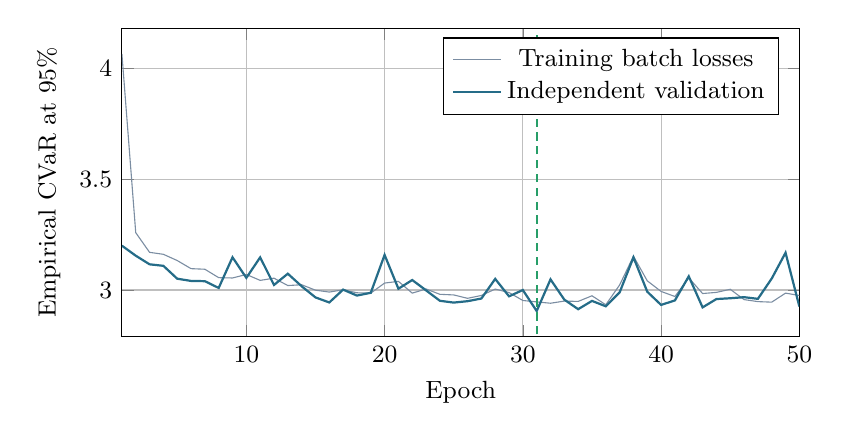
\begin{tikzpicture}
\begin{axis}[width=.84\linewidth,height=5.5cm,xlabel={Epoch},ylabel={Empirical CVaR at 95\%},
 xmin=1,xmax=50,grid=major,legend style={font=\small,at={(.97,.97)},anchor=north east},
 tick label style={font=\small},label style={font=\small}]
\addplot[plotslate,thin] coordinates {
(1,4.065190709)
(2,3.25890555)
(3,3.17018717)
(4,3.161273219)
(5,3.133132578)
(6,3.09650489)
(7,3.093874539)
(8,3.055868758)
(9,3.054401928)
(10,3.070329005)
(11,3.04359568)
(12,3.053498421)
(13,3.020257787)
(14,3.02393157)
(15,2.999426648)
(16,2.990888544)
(17,3.001068785)
(18,2.987651511)
(19,2.98605945)
(20,3.031493555)
(21,3.039159519)
(22,2.98611018)
(23,3.004794465)
(24,2.980733675)
(25,2.977924492)
(26,2.962667001)
(27,2.975563215)
(28,3.004375814)
(29,2.988715131)
(30,2.952856429)
(31,2.946564503)
(32,2.94050616)
(33,2.950187501)
(34,2.948677906)
(35,2.974122054)
(36,2.933561472)
(37,3.022983731)
(38,3.152566178)
(39,3.041488127)
(40,2.993653831)
(41,2.970850763)
(42,3.055097268)
(43,2.984284217)
(44,2.989457519)
(45,3.003434512)
(46,2.956920771)
(47,2.947787754)
(48,2.945344936)
(49,2.986113357)
(50,2.97540288)
};\addlegendentry{Training batch losses}
\addplot[plotblue,thick] coordinates {
(1,3.200148697)
(2,3.155010407)
(3,3.116086778)
(4,3.109222851)
(5,3.051216376)
(6,3.041097089)
(7,3.040014463)
(8,3.009437924)
(9,3.147799026)
(10,3.054979568)
(11,3.147405079)
(12,3.022926588)
(13,3.07380065)
(14,3.01715545)
(15,2.966786659)
(16,2.943984279)
(17,3.001894311)
(18,2.975042457)
(19,2.987683219)
(20,3.158379289)
(21,3.005930525)
(22,3.045245923)
(23,2.998568471)
(24,2.951516206)
(25,2.943398149)
(26,2.949705912)
(27,2.961781753)
(28,3.050301877)
(29,2.971673878)
(30,3.000120826)
(31,2.905225508)
(32,3.048204087)
(33,2.956632536)
(34,2.913611563)
(35,2.950984372)
(36,2.926673799)
(37,2.989492564)
(38,3.147628847)
(39,2.992327852)
(40,2.932781182)
(41,2.953400337)
(42,3.06186796)
(43,2.921797005)
(44,2.959445853)
(45,2.962989265)
(46,2.967813758)
(47,2.960314315)
(48,3.051836013)
(49,3.168413506)
(50,2.925704356)
};\addlegendentry{Independent validation}
\draw[plotgreen,thick,densely dashed] (axis cs:31,2.8)--(axis cs:31,4.15);
\end{axis}
\end{tikzpicture}
\caption{The completed independent 50-epoch run. Training values collect losses while parameters change within an epoch; validation values evaluate the fixed policy after each epoch. The green dashed line marks the selected epoch. This is not an original-paper training figure.}
\label{fig:training}
\end{figure}

\section{Conditional delta and deterministic evaluation}
\subsection{Delta as a conditional expectation}
Fix a decision date $t$, a strictly positive current spot $s$, a strictly positive current variance $h$, and $\tau=T-t\geq1$. With parameters and $h$ held fixed, the future variance transitions and innovation laws do not depend on $s$. The terminal stock may therefore be written
\begin{equation}
 S_T=sM,\qquad
 M=\exp\!\left(\sum_{j=t}^{T-1}R_{j+1}\right)>0.
\end{equation}
The law of $M$ depends on $h$ and $\tau$, but not on $s$. Equation~\eqref{eq:qfirstmomentsteps} gives $\E_{\Q}[M\mid h_t=h]=e^{c\tau}<\infty$. The conditional option price is
\begin{equation}
 C_\tau(s,h)=e^{-r\tau\dt}\E_{\Q}[(sM-K)^+\mid h_t=h].
\end{equation}
The function $v\mapsto v^+$ is 1-Lipschitz, so for any non-zero bump $b$ with $s+b>0$,
\begin{equation}
 \left|\frac{((s+b)M-K)^+-(sM-K)^+}{b}\right|
 \leq \frac{|bM|}{|b|}=M.
\end{equation}
The difference quotient tends to $M\ind_{\{sM>K\}}$ except on $\{sM=K\}$. That exceptional event has zero probability: conditionally on $\F_{T-1}$, the final log stock is Gaussian with strictly positive variance $h_{T-1}$, so
\begin{equation}
 \Q(S_T=K\mid\F_{T-1})=0,
 \qquad
 \Q(S_T=K\mid\F_t)=
 \E_{\Q}[\Q(S_T=K\mid\F_{T-1})\mid\F_t]=0.
\end{equation}
The integrable dominating variable $M$ now permits differentiation under the expectation. Evaluating at the observed state gives the paper's Equation~(9):
\begin{equation}
 \Delta_t=\frac{\partial C_\tau}{\partial s}(S_t,h_t)
 =e^{-r\tau\dt}\E_{\Q}\!\left[
        \frac{S_T}{S_t}\ind_{\{S_T>K\}}\mid\F_t\right].
 \label{eq:delta}
\end{equation}
This is a partial derivative with current variance held fixed. No physical-measure payoff moment is required for this pricing-measure differentiation.

\subsection{Total-return-stock measure}
The total-return stock is $N_t=e^{qt\dt}S_t$ and the money account is $B_t=e^{rt\dt}$. Their ratio $N_t/B_t=e^{-ct}S_t$ is the positive martingale established above. Normalise it by its initial value:
\begin{equation}
 Z_t^S=\frac{N_t/B_t}{N_0/B_0}
      =e^{-ct}\frac{S_t}{S_0},\qquad
 \E_{\Q}[Z_t^S]=1.
\end{equation}
Define $d\Q^S/d\Q=Z_T^S$ on $\F_T$. Conditional Bayes' formula gives, for a bounded terminal random variable $A$,
\begin{align}
 \E_{\Q^S}[A\mid\F_t]
 &=\frac{\E_{\Q}[Z_T^SA\mid\F_t]}{Z_t^S}\nonumber\\
 &=\E_{\Q}\!\left[
     e^{-c\tau}\frac{S_T}{S_t}A\mid\F_t\right].
 \label{eq:stockmeasure}
\end{align}
Taking $A=\ind_{\{S_T>K\}}$ and rearranging \eqref{eq:delta} gives
\begin{align}
 \Delta_t
 &=e^{-r\tau\dt}e^{c\tau}\E_{\Q^S}[\ind_{\{S_T>K\}}\mid\F_t]\nonumber\\
 &=e^{-q\tau\dt}\Q^S(S_T>K\mid\F_t),\qquad
 0\leq\Delta_t\leq e^{-q\tau\dt}.
 \label{eq:probdelta}
\end{align}
This replaces the potentially high-variance terminal stock-ratio weight with a bounded exercise probability.

The one-period conditional density factor is
\begin{equation}
 \frac{Z_{t+1}^S}{Z_t^S}
 =e^{-c}\frac{S_{t+1}}{S_t}
 =\exp(\sqrt{h_t}Z_{t+1}-h_t/2).
\end{equation}
Multiplying the standard $\Q$ normal density and completing the square yields
\begin{align}
 \varphi(z)e^{\sqrt h z-h/2}
 &=\frac1{\sqrt{2\pi}}\exp[-z^2/2+\sqrt h z-h/2]\nonumber\\
 &=\frac1{\sqrt{2\pi}}\exp[-(z-\sqrt h)^2/2]
 =\varphi(z-\sqrt h).
\end{align}
Thus $Z_{t+1}=\sqrt{h_t}+u_{t+1}$, where $u_{t+1}$ is conditionally standard normal under $\Q^S$. These centred conditional laws are independent of the past. Repeating this step is the full stock-measure change, because
\begin{equation}
 \prod_{j=t}^{T-1}\frac{Z_{j+1}^S}{Z_j^S}
 =\frac{Z_T^S}{Z_t^S}=e^{-c\tau}\frac{S_T}{S_t}.
\end{equation}
The variance remains the same pathwise function of the physical innovation. That innovation is
\begin{equation}
 \varepsilon_{t+1}=Z_{t+1}-\eta_t
                 =u_{t+1}+\sqrt{h_t}-\eta_t,
\end{equation}
so neither the leverage indicator nor the squared shock may be replaced by $u_{t+1}$ alone. Writing $x=\log(S/K)$ and $\eta(h)=(\mu-c+h/2)/\sqrt h$, the resulting transitions are
\begin{align}
 x'(u)&=x+c-h/2+\sqrt h(\sqrt h+u)
       =x+c+h/2+\sqrt h\,u,\nonumber\\
 h'(u)&=\omega+h[\alpha+\gamma\ind_{\{u+\sqrt h-\eta(h)<0\}}]
                    (u+\sqrt h-\eta(h))^2+\beta h.
 \label{eq:stocktransition}
\end{align}
These are transitions of the pair $(x,h)$ under $\Q^S$. Their future law depends only on this pair and the fixed parameters, which supplies the Markov property used below.

\subsection{Backward recursion and quadrature}
Let $p_\tau(x,h)$ be the stock-measure probability that the terminal log moneyness is positive, with $\tau$ days remaining. At maturity,
\begin{equation}
 p_0(x,h)=\ind_{\{x>0\}}.
\end{equation}
For one remaining day, the exercise event is
\begin{equation}
 x+c+h/2+\sqrt h\,u>0
 \quad\Longleftrightarrow\quad
 u>-\frac{x+c+h/2}{\sqrt h}.
\end{equation}
Normal symmetry therefore gives
\begin{equation}
 p_1(x,h)=1-\Phi\!\left(-\frac{x+c+h/2}{\sqrt h}\right)
          =\Phi\!\left(\frac{x+c+h/2}{\sqrt h}\right),\qquad
 \Delta_1(S,h)=e^{-q\dt}p_1(\log(S/K),h).
\end{equation}
This analytic starting surface avoids applying quadrature directly to the terminal discontinuity. The implementation also uses this exact one-day expression for every off-grid evaluation state.

For $\tau\geq2$, apply the tower property, then the Markov property, then the conditional normal law of $u$:
\begin{align}
 p_\tau(x,h)
 &=\E_{\Q^S}[\ind_{\{x_T>0\}}\mid x_t=x,h_t=h]\nonumber\\
 &=\E_{\Q^S}\!\left[
     \E_{\Q^S}[\ind_{\{x_T>0\}}\mid x_{t+1},h_{t+1}]
       \mid x_t=x,h_t=h\right]\nonumber\\
 &=\E_{\Q^S}[p_{\tau-1}(x'(u),h'(u))]\nonumber\\
 &=\int_{\mathbb R}p_{\tau-1}(x'(u),h'(u))
       \frac{e^{-u^2/2}}{\sqrt{2\pi}}\,du,\nonumber\\
 \Delta_\tau(S,h)&=e^{-q\tau\dt}p_\tau(\log(S/K),h).
 \label{eq:backward}
\end{align}
Every integrand is bounded between zero and one, so these conditional expectations and iterated integrals are well defined.

The probabilists' Hermite polynomial is
\begin{equation}
 H_n(u)=(-1)^ne^{u^2/2}\frac{d^n}{du^n}e^{-u^2/2}.
\end{equation}
Write $\rho(u)=e^{-u^2/2}$. For a polynomial $v$ of degree below $n$, Rodrigues' formula and $n$ integrations by parts give
\begin{equation}
 \int_{\mathbb R}H_n(u)v(u)\rho(u)\,du
 =(-1)^n\int_{\mathbb R}v(u)\rho^{(n)}(u)\,du
 =\int_{\mathbb R}v^{(n)}(u)\rho(u)\,du=0.
\end{equation}
All boundary terms vanish because a Gaussian density and its derivatives dominate any polynomial at infinity. Orthogonality also explains why $H_n$ has $n$ distinct real roots: otherwise let $v$ be the product of its real roots at which the sign changes. Its degree would be below $n$, while $H_nv$ would have one constant non-zero sign except at finitely many points, contradicting the zero integral above. Denote these roots by $u_1,\ldots,u_n$.

Define the Lagrange polynomials and weights by
\begin{equation}
 \ell_k(u)=\frac{H_n(u)}{(u-u_k)H_n'(u_k)},\qquad
 \ell_k(u_j)=\ind_{\{k=j\}},\qquad
 W_k=\int_{\mathbb R}\ell_k(u)\rho(u)\,du.
\end{equation}
For a polynomial $f$ of degree at most $2n-1$, polynomial division gives $f=H_n v+r$ with $\deg(v)\leq n-1$ and $\deg(r)\leq n-1$. Orthogonality removes the first term from the integral. Since $r(u_k)=f(u_k)$, interpolation of $r$ gives
\begin{align}
 \int_{\mathbb R}f(u)\rho(u)\,du
 &=\int_{\mathbb R}r(u)\rho(u)\,du\nonumber\\
 &=\int_{\mathbb R}\sum_{k=1}^nf(u_k)\ell_k(u)\rho(u)\,du
 =\sum_{k=1}^nW_kf(u_k).
\end{align}
Applying this identity to $f=\ell_k^2$, whose degree is $2n-2$, proves positivity:
\begin{equation}
 W_k=\sum_{j=1}^nW_j\ell_k(u_j)^2
 =\int_{\mathbb R}\ell_k(u)^2\rho(u)\,du>0.
\end{equation}

The explicit weight formula can be recovered from the same identities. The monic Hermite polynomial $H_m$ has degree $m$, so integration by parts gives
\begin{equation}
 \int_{\mathbb R}H_m(u)^2\rho(u)\,du
 =\int_{\mathbb R}H_m^{(m)}(u)\rho(u)\,du
 =m!\sqrt{2\pi}.
\end{equation}
Rodrigues' formula gives $H_n'=nH_{n-1}$. Moreover $\ell_k$ has leading coefficient $1/H_n'(u_k)$; hence $\ell_k-H_{n-1}/H_n'(u_k)$ has degree at most $n-2$. Orthogonality and quadrature exactness for $\ell_kH_{n-1}$ therefore imply
\begin{align}
 W_kH_{n-1}(u_k)
 &=\int_{\mathbb R}\ell_k(u)H_{n-1}(u)\rho(u)\,du\nonumber\\
 &=\frac{1}{H_n'(u_k)}
       \int_{\mathbb R}H_{n-1}(u)^2\rho(u)\,du
 =\frac{(n-1)!\sqrt{2\pi}}{nH_{n-1}(u_k)}.
\end{align}
Since $H_n'(u_k)\ne0$, division yields
\begin{equation}
 W_k=\frac{\sqrt{2\pi}\,n!}{n^2H_{n-1}(u_k)^2}.
\end{equation}
Applying the polynomial identity to $f\equiv1$ gives $\sum_kW_k=\sqrt{2\pi}$. Thus $w_k=W_k/\sqrt{2\pi}$ are normal-expectation weights with $w_k>0$ and $\sum_kw_k=1$. The implementation obtains the nodes and raw weights from \texttt{roots\_hermitenorm(48)} and performs this normalisation. The exercise-probability integrand is not a polynomial, so the 48-node expression is a numerical approximation rather than an exact integration statement.

For the grid, write $y=\log h$, $h_j=e^{y_j}$, and let $\widetilde p_{\tau,j,i}$ denote the stored approximation at $(x_i,h_j)$. The initial arrays are
\begin{equation}
 \widetilde p_{0,j,i}=\ind_{\{x_i>0\}},\qquad
 \widetilde p_{1,j,i}=\Phi\!\left(\frac{x_i+c+h_j/2}{\sqrt{h_j}}\right).
\end{equation}
To evaluate a preceding surface between grid points, suppose $x_i\leq x\leq x_{i+1}$ and $y_j\leq y\leq y_{j+1}$. Define
\begin{equation}
 b=\frac{x-x_i}{x_{i+1}-x_i},\qquad
 a_y=\frac{y-y_j}{y_{j+1}-y_j}.
\end{equation}
First interpolate within each adjacent variance row,
\begin{equation}
 \ell_j(x)=(1-b)p_{j,i}+bp_{j,i+1},\qquad
 \ell_{j+1}(x)=(1-b)p_{j+1,i}+bp_{j+1,i+1},
\end{equation}
and then interpolate between rows:
\begin{align}
 \mathcal I[p](x,y)
 &=(1-a_y)\ell_j(x)+a_y\ell_{j+1}(x)\nonumber\\
 &=(1-a_y)[(1-b)p_{j,i}+bp_{j,i+1}]
   +a_y[(1-b)p_{j+1,i}+bp_{j+1,i+1}].
 \label{eq:interpolation}
\end{align}
Combining this spatial approximation with the quadrature rule gives the actual backward update, for $\tau=2,\ldots,T$:
\begin{equation}
 \widetilde p_{\tau,j,i}
 =\sum_{k=1}^{48}w_k\,
   \mathcal I[\widetilde p_{\tau-1}]
       \bigl(x'_{i,j}(u_k),\log h'_j(u_k)\bigr).
 \label{eq:quadrature}
\end{equation}
Within a grid cell, the four interpolation coefficients are non-negative and sum to one. The quadrature weights have the same properties. Hence bounded preceding values produce a value in $[0,1]$ in exact arithmetic; the code clips round-off to this interval. The transition is evaluated separately at each quadrature node, including the shifted leverage indicator. The fine and wide grids each construct their own complete backward surfaces; the evaluation selects the wide result when the current state has $h>0.01$, and otherwise selects the fine result. This is a choice between two numerical approximations of the same conditional delta, rather than a change of the financial model.

The surfaces and precomputed interpolation fractions are stored in float32. Bilinear interpolation during backward construction consequently uses float32; each quadrature-weighted contribution and its accumulation use float64. Final interpolation at the requested off-grid financial states uses float64. The final one-day delta is evaluated analytically instead of interpolating the stored one-day surface. Domain truncation, grid interpolation, quadrature and floating-point rounding are separate numerical errors; the following tables and conditional-simulation checks assess their practical effect without supplying a global error bound.

\begin{table}[htbp]
\centering\small
\caption{Numerical probability grids. The wide grid supplies evaluation states with $h>0.01$.}
\label{tab:grids}
\begin{tabular}{@{}llll@{}}
\toprule
Grid & Log moneyness $x$ & Log variance $y$ & Normal quadrature\\
\midrule
Fine & $[-1.5,1.5]$, 4,801 points & $[-12,-1]$, 221 points & 48 nodes\\
Wide & $[-4,4]$, 1,601 points & $[-12,3]$, 301 points & 48 nodes\\
\bottomrule
\end{tabular}
\end{table}
Fine spacings are 0.000625 in $x$ and 0.05 in $y$; wide spacings are 0.005 and 0.05. Outside the moneyness domain the exercise probability is approximated by zero or one, and out-of-domain log variance is clipped to the nearest endpoint. These are numerical boundary approximations. Since $h'\geq\omega+\beta h$, the interval $[\omega/(1-\beta),\infty)$ is invariant. Its lower endpoint is $1.348048044358411\times 10^{-5}$, above the grid lower bound $e^{-12}$. The final physical current-state range lies inside the fine domain, while the wide grid improves large-variance future excursions. I inspect evaluation-path state extremes for numerical coverage only; neither policy nor parameters are fitted to test losses. Transition boundary errors remain numerical uncertainty.

The completed test contains 6.3 million decision states: 6.2 million interpolated deltas and 100,000 analytical one-day deltas. The fine-grid audit records no current-state moneyness or variance clamps; the wide grid supplies 210 states with $h>0.01$. The deterministic recursion replaces the authors' 1,000-path nested conditional Monte Carlo calculation. It estimates the same mathematical delta through a different numerical procedure.

\subsection{Resolution and conditional-simulation checks}
\begin{table}[htbp]
\centering\small
\caption{Final-grid comparisons with independent conditional simulation. The last column is $(\Delta_{\rm grid}-\Delta_{\rm MC})/\SE_{\rm MC}$. Wide-domain values are used for the high-variance states.}
\label{tab:deltachecks}
\begin{tabular}{@{}rrlrrrr@{}}
\toprule
$\tau$ & $S$ & $h$ & Grid delta & MC delta & MC SE & Difference/SE\\
\midrule
63 & 100.000 & $2.6666\times 10^{-5}$ & 0.565140 & 0.564975 & 0.000650 & 0.26 \\
31 & 95.000 & $4\times 10^{-5}$ & 0.112151 & 0.111599 & 0.000394 & 1.40 \\
10 & 105.000 & $0.00015$ & 0.907277 & 0.906977 & 0.000334 & 0.90 \\
2 & 100.000 & $3\times 10^{-5}$ & 0.512321 & 0.511961 & 0.000390 & 0.92 \\
63 & 100.000 & $0.001$ & 0.594539 & 0.594389 & 0.000664 & 0.23 \\
16 & 78.881 & $0.049961$ & 0.541694 & 0.542079 & 0.000634 & -0.61 \\
7 & 45.761 & $0.078222$ & 0.192775 & 0.192087 & 0.000454 & 1.52 \\
63 & 100.000 & $2.6083\times 10^{-5}$ & 0.565089 & 0.565649 & 0.000490 & -1.14 \\
38 & 80.000 & $0.012$ & 0.422406 & 0.421303 & 0.000666 & 1.66 \\
\bottomrule
\end{tabular}
\end{table}
The largest absolute difference in Table~\ref{tab:deltachecks} is 0.001103033, and the largest absolute standardised difference is 1.657. Ordinary and wide-state comparisons use 500,000 paths; the initial direct-$\Q$ comparison uses one million paths. The additional out-of-the-money comparison uses two million stock-measure paths, seed~69342, giving $0.111822219$ with SE $0.000197114$. Stock-measure comparisons estimate bounded indicator probabilities, while the direct-$\Q$ comparison is retained as an empirical diagnostic without a proven finite second moment of its stock-ratio weight.

\begin{table}[htbp]
\centering\small
\caption{Spot-resolution refinement diagnostics from the recorded calibration. ``Fine'' and ``refined'' denote the paired grids in the resolution check, not a new trained policy.}
\label{tab:refinement}
\begin{tabular}{@{}rrlrrr@{}}
\toprule
$\tau$ & $S$ & $h$ & Fine delta & Refined delta & Refined minus fine\\
\midrule
63 & 100.000 & $2.6083\times 10^{-5}$ & 0.564875 & 0.565088 & +0.000212 \\
63 & 100.000 & $2.6666\times 10^{-5}$ & 0.564928 & 0.565140 & +0.000211 \\
31 & 95.000 & $4\times 10^{-5}$ & 0.112620 & 0.112151 & -0.000469 \\
10 & 105.000 & $0.00015$ & 0.907176 & 0.907277 & +0.000100 \\
2 & 100.000 & $3\times 10^{-5}$ & 0.512330 & 0.512321 & -0.000009 \\
63 & 100.000 & $0.001$ & 0.594409 & 0.594467 & +0.000058 \\
\bottomrule
\end{tabular}
\end{table}
The largest change is $0.000468611$. In the constant-volatility specialisation, the same recursion is checked against the analytical Black--Scholes delta:
\begin{table}[htbp]
\centering\small
\caption{Constant-volatility check with daily variance $h=0.00012340980408667956$.}
\begin{tabular}{@{}rrrrr@{}}
\toprule
$\tau$ & $S$ & Grid delta & Analytical delta & Grid minus analytical\\
\midrule
63 & 100 & 0.515658 & 0.515677 & -0.0000192 \\
63 & 95 & 0.294594 & 0.294394 & +0.0002004 \\
31 & 105 & 0.792072 & 0.792322 & -0.0002500 \\
2 & 100 & 0.503112 & 0.503108 & +0.0000041 \\
1 & 100 & 0.502212 & 0.502212 & +0.0000000 \\
\bottomrule
\end{tabular}
\end{table}
The largest recorded difference is $0.000250048$; the one-day formula agrees exactly. These checks support the selected resolution but are not a uniform error bound for all states or for the resulting hedge statistics.

\section{Test results and empirical uncertainty}
\subsection{Fixed-policy evaluation}
I load the selected checkpoint and evaluate it without gradient updates on seed-45 paths. I compute its positions in float32, in batches of 1,000. For the reported statistics, I accumulate both base wealth processes and the overlay in float64 using these fixed positions and the stored float32 market gains and payoff. The per-path records are
\begin{equation}
 L_i^{\rm DH}=H_i-V_{T,i}^{\rm DH},\qquad
 L_i^\Delta=H_i-V_{T,i}^\Delta,\qquad L_i^-=-U_{T,i}.
\end{equation}
Each empirical CVaR is the mean of the largest 5,000 losses among $n=100,000$ outcomes. The gap is a difference of two separately computed tail risks, rather than CVaR of the difference:
\begin{equation}
 \widehat G=\widehat{\CVaR}_a(L^{\rm DH})-\widehat{\CVaR}_a(L^\Delta),
 \qquad \widehat{\CVaR}_a(L^-)\ne\widehat G\quad\hbox{in general}.
\end{equation}

\begin{table}[htbp]
\centering\footnotesize
\caption{Published 95\% benchmarks from Table~1 and the independent run. The published values are transcribed reference statistics; the independent column contains this experiment. Intervals are conditional empirical plug-in intervals, with unestablished population coverage as discussed below.}
\label{tab:results}
\begin{tabular}{@{}lrrrr@{}}
\toprule
Statistic & Published & Independent & Plug-in SE & 95\% plug-in interval\\
\midrule
$\widehat{\operatorname{CVaR}}_a(L^{\rm DH})$ & 3.481 & 2.884726 & 0.048019 & $[2.7906,2.9788]$ \\
$\widehat{\operatorname{CVaR}}_a(L^{\rm DH})-\widehat{\operatorname{CVaR}}_a(L^\Delta)$ & -0.081 & -0.075220 & 0.038560 & $[-0.1508,0.0004]$ \\
$\widehat{\operatorname{CVaR}}_a(-U_T)$ & 1.810 & 1.865054 & 0.026827 & $[1.8125,1.9176]$ \\
$\overline U_T$ & -0.254 & -0.262780 & 0.003372 & $[-0.2694,-0.2562]$ \\
\bottomrule
\end{tabular}
\end{table}
The four independent-minus-published differences, in row order, are $-0.596274$, $+0.005780$, $+0.055054$, $-0.008780$. The published implied delta CVaR is $3.481-(-0.081)=3.562$; the independent delta CVaR is 2.959945763. The independent overlay has positive empirical loss CVaR and negative mean profit. It therefore does not meet the paper's CVaR statistical-arbitrage criterion in this sample, matching the signs of its published 95\% result. Its exact figures are not reproduced. The estimated deep-minus-delta gap is negative, but its plug-in interval includes zero; an improvement is not resolved at that sampling precision. The published statistics have their own unreported simulation uncertainty, so comparison with rounded published values is not a formal significance test.

\subsection{Influence-function calculation}
Let $F$ be a continuous loss distribution, $p=1-a$, $q_a$ its $a$-quantile and
$C=q_a+\E_F[(L-q_a)^+]/p$. This derivation is conditional on the regularity and moments needed for a population influence function; it does not establish them for the actual hedge losses.

To compute the first-order effect of one observation $l$, contaminate the law by
$F_\epsilon=(1-\epsilon)F+\epsilon\delta_l$, and denote its quantile and CVaR by $q_\epsilon$ and $C_\epsilon$. Here $\delta_l$ is point mass at the loss $l$, not a hedge position. Assuming a positive density $f(q_a)$ and $l\ne q_a$, differentiate the quantile equation:
\begin{align}
 (1-\epsilon)F(q_\epsilon)+\epsilon\ind_{\{l\leq q_\epsilon\}}&=a,\nonumber\\
 -F(q_a)+f(q_a)\dot q+\ind_{\{l\leq q_a\}}&=0,\nonumber\\
 \dot q:=\left.\frac{dq_\epsilon}{d\epsilon}\right|_0
 &=\frac{a-\ind_{\{l\leq q_a\}}}{f(q_a)}.
\end{align}
Write out the contaminated tail objective before differentiating:
\begin{equation}
 C_\epsilon=q_\epsilon+\frac1p\left\{
 (1-\epsilon)\E_F[(L-q_\epsilon)^+]
       +\epsilon(l-q_\epsilon)^+\right\}.
\end{equation}
The derivative of $\E_F[(L-q)^+]$ with respect to $q$ is
$-\Pp_F(L>q)$. Product and chain rules therefore give
\begin{align}
 \IF_C(l):=\left.\frac{dC_\epsilon}{d\epsilon}\right|_0
 &=\dot q+\frac1p\left\{
   -\E_F[(L-q_a)^+]-\dot q\,\Pp_F(L>q_a)
                    +(l-q_a)^+\right\}\nonumber\\
 &=\dot q\left(1-\frac p p\right)
   +\frac{(l-q_a)^+-\E_F[(L-q_a)^+]}p\nonumber\\
 &=\frac{(l-q_a)^+}{1-a}
   -\E_F\!\left[\frac{(L-q_a)^+}{1-a}\right]\nonumber\\
 &=q_a+\frac{(l-q_a)^+}{1-a}-C.
 \label{eq:influence}
\end{align}
The quantile derivative cancels because $\Pp_F(L>q_a)=p$ at the optimum. In particular $\E_F[\IF_C(L)]=0$. Under the stated regularity and moment assumptions, the first-order sample expansion is
\begin{equation}
 \widehat C-C=\frac1n\sum_{i=1}^n\IF_C(L_i)+o_{\Pp}(n^{-1/2}).
\end{equation}
For independent test paths, the variance of this first-order average is
\begin{equation}
 \Var\!\left(\frac1n\sum_{i=1}^n\IF_C(L_i)\right)
 =\frac{n\Var(\IF_C(L))}{n^2}
 =\frac{\Var(\IF_C(L))}{n}.
\end{equation}
Replacing the unknown influence-function variance by its sample variance and taking the square root gives \eqref{eq:cvarinterval}.
The implemented empirical quantile is the order statistic at zero-based index $\lfloor an\rfloor$. Taking the adjacent empirical minimiser gives the same top-5\% CVaR. For each observation the code computes $z_i=(L_i-q_a)^+/(1-a)$ and centres it by its sample mean. Its plug-in interval is
\begin{equation}
 \widehat{\SE}(\widehat C)=\frac{\sd_{n-1}(\widehat{\IF}_{C,i})}{\sqrt n},
 \qquad \widehat C\pm1.96\widehat{\SE}(\widehat C).
 \label{eq:cvarinterval}
\end{equation}
Because both hedges use the same test paths, gap uncertainty is paired:
\begin{align}
 \IF_{G,i}&=\IF_{{\rm DH},i}-\IF_{\Delta,i},\nonumber\\
 \Var(\IF_G)&=\Var(\IF_{\rm DH})+\Var(\IF_\Delta)-2\Cov(\IF_{\rm DH},\IF_\Delta),\nonumber\\
 \widehat{\SE}(\widehat G)&=\frac{\sd_{n-1}(\widehat{\IF}_{G,i})}{\sqrt n},
 &\widehat{\SE}(\overline U_T)&=\frac{\sd_{n-1}(U_{T,i})}{\sqrt n}.
 \label{eq:pairedse}
\end{align}
This retains the covariance that an independent-samples calculation would discard. The overlay mean interval is $\overline U_T\pm1.96\widehat{\SE}(\overline U_T)$.

These calculations condition on one selected policy, the retained calibration and the numerical delta benchmark. They exclude calibration, repeat-training and quadrature uncertainty. A normal central limit approximation additionally requires a finite second moment of the relevant influence function, plus quantile regularity. Those population assumptions are not proved for the hedge losses or overlay; the result below makes this qualification material. Table~\ref{tab:results} therefore records finite-Monte-Carlo-sample empirical risks and means with plug-in uncertainty, rather than established population confidence coverage.

\subsection{Reconstructed distribution}
For the central panel, set $b_j=-5+0.1j$, $j=0,\ldots,100$. With $U_i=U_{T,i}$, the height of bin $j$ is
\begin{equation}
 N_j=\sum_{i=1}^{100,000}\ind_{\{b_{j-1}\leq U_i<b_j\}},
 \qquad j=1,\ldots,100,
\end{equation}
with the final upper endpoint included in the last bin. Bars are located at the midpoints $(b_{j-1}+b_j)/2$. The bin counts sum to 99,756, leaving $100,000-99,756=244$ outcomes outside the central range. For the full panel, use edges $a_j=U_{\min}+j(U_{\max}-U_{\min})/100$ and the same counting rule; its counts sum to 100,000. The logarithmic frequency axis changes the displayed height scale, while preserving these counts.


The exported counts are in \texttt{figure1\_histogram.csv}; the observed minimum and maximum are $-40.253998$ and $21.435711$. All outcomes enter the statistics.
\begin{figure}[htbp]
\centering
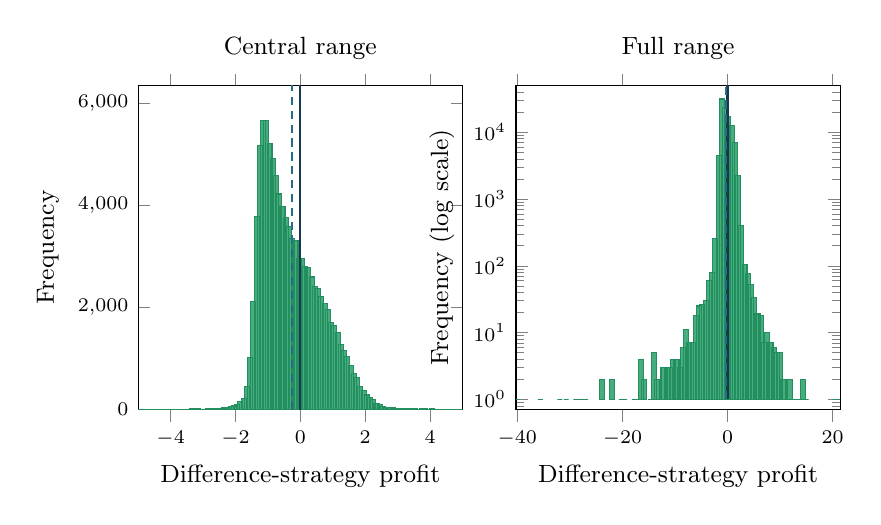
\begin{tikzpicture}
\begin{axis}[name=central,width=.47\linewidth,height=5.7cm,
 xlabel={Difference-strategy profit},ylabel={Frequency},title={Central range},
 xmin=-5,xmax=5,ymin=0,ymax=6354,ybar,bar width=1.8pt,
 tick label style={font=\scriptsize},label style={font=\small},title style={font=\small}]
\addplot[fill=plotgreen!85,draw=plotgreen!90!black] coordinates {
(-4.95,4)
(-4.85,5)
(-4.75,3)
(-4.65,4)
(-4.55,3)
(-4.45,4)
(-4.35,5)
(-4.25,7)
(-4.15,4)
(-4.05,4)
(-3.95,4)
(-3.85,8)
(-3.75,7)
(-3.65,8)
(-3.55,12)
(-3.45,8)
(-3.35,13)
(-3.25,15)
(-3.15,14)
(-3.05,4)
(-2.95,7)
(-2.85,15)
(-2.75,21)
(-2.65,14)
(-2.55,26)
(-2.45,30)
(-2.35,34)
(-2.25,39)
(-2.15,55)
(-2.05,72)
(-1.95,104)
(-1.85,153)
(-1.75,217)
(-1.65,449)
(-1.55,1015)
(-1.45,2123)
(-1.35,3787)
(-1.25,5182)
(-1.15,5673)
(-1.05,5668)
(-0.95,5224)
(-0.85,4923)
(-0.75,4596)
(-0.65,4227)
(-0.55,3988)
(-0.45,3771)
(-0.35,3586)
(-0.25,3347)
(-0.15,3310)
(-0.05,2961)
(0.05,2959)
(0.15,2804)
(0.25,2784)
(0.35,2601)
(0.45,2421)
(0.55,2372)
(0.65,2212)
(0.75,2084)
(0.85,1963)
(0.95,1710)
(1.05,1658)
(1.15,1518)
(1.25,1284)
(1.35,1160)
(1.45,1045)
(1.55,869)
(1.65,704)
(1.75,630)
(1.85,456)
(1.95,385)
(2.05,289)
(2.15,236)
(2.25,201)
(2.35,118)
(2.45,100)
(2.55,71)
(2.65,43)
(2.75,38)
(2.85,35)
(2.95,29)
(3.05,21)
(3.15,20)
(3.25,14)
(3.35,11)
(3.45,14)
(3.55,13)
(3.65,12)
(3.75,13)
(3.85,16)
(3.95,5)
(4.05,19)
(4.15,5)
(4.25,8)
(4.35,10)
(4.45,10)
(4.55,12)
(4.65,5)
(4.75,7)
(4.85,8)
(4.95,1)
};
\draw[plotink,thick] (axis cs:0,0)--(axis cs:0,6354);
\draw[plotblue,thick,densely dashed] (axis cs:-0.2627795269,0)--(axis cs:-0.2627795269,6354);
\end{axis}
\begin{axis}[at={(central.east)},anchor=west,xshift=.68cm,width=.47\linewidth,height=5.7cm,
 xlabel={Difference-strategy profit},ylabel={Frequency (log scale)},title={Full range},
 xmin=-40.253998146,xmax=21.435711138,ymode=log,ymin=.7,ymax=50194,
 ybar,bar width=1.8pt,
 tick label style={font=\scriptsize},label style={font=\small},title style={font=\small}]
\addplot[fill=plotgreen!85,draw=plotgreen!90!black] coordinates {
(-39.9455496,1)
(-35.62726995,1)
(-31.92588739,1)
(-30.69209321,1)
(-28.84140193,1)
(-28.22450484,1)
(-27.60760774,1)
(-26.99071065,1)
(-23.90622519,2)
(-22.05553391,2)
(-20.20484263,1)
(-19.58794554,1)
(-17.73725426,1)
(-17.12035716,1)
(-16.50346007,4)
(-15.88656298,2)
(-14.65276879,1)
(-14.0358717,5)
(-13.41897461,2)
(-12.80207751,1)
(-12.18518042,3)
(-11.56828333,3)
(-10.95138624,3)
(-10.33448914,4)
(-9.717592051,4)
(-9.100694958,3)
(-8.483797865,6)
(-7.866900772,11)
(-7.250003679,7)
(-6.633106586,7)
(-6.016209493,18)
(-5.399312401,25)
(-4.782415308,26)
(-4.165518215,30)
(-3.548621122,60)
(-2.931724029,79)
(-2.314826936,256)
(-1.697929843,4421)
(-1.081032751,31371)
(-0.4641356578,23726)
(0.152761435,17436)
(0.7696585279,12536)
(1.386555621,6936)
(2.003452714,2233)
(2.620349806,405)
(3.237246899,106)
(3.854143992,77)
(4.471041085,53)
(5.087938178,34)
(5.704835271,19)
(6.321732364,18)
(6.938629456,7)
(7.555526549,10)
(8.172423642,7)
(8.789320735,6)
(9.406217828,5)
(10.02311492,5)
(10.64001201,2)
(11.25690911,1)
(11.8738062,2)
(12.49070329,1)
(13.10760038,1)
(13.72449748,1)
(14.34139457,2)
(14.95829166,1)
(20.5103655,1)
(21.12726259,1)
};
\draw[plotink,thick] (axis cs:0,1)--(axis cs:0,50194);
\draw[plotblue,thick,densely dashed] (axis cs:-0.2627795269,1)--(axis cs:-0.2627795269,50194);
\end{axis}
\end{tikzpicture}
\caption{Independently simulated distribution corresponding to the paper's 95\% experiment; these are not the original Figure~1 data. Both panels contain the same test sample. The blue dashed line marks the mean; the solid line marks zero. Only the displayed central panel excludes the 244 out-of-range observations.}
\label{fig:distribution}
\end{figure}
The supplied \texttt{terminal\_results.npz} preserves every deep loss, delta loss and overlay profit. Selected empirical profit quantiles are
\begin{center}\small
\begin{tabular}{@{}rr@{}}\toprule
Probability & Overlay profit quantile\\\midrule
0.001 & -5.695278 \\
0.010 & -1.721078 \\
0.050 & -1.389416 \\
0.500 & -0.444564 \\
0.950 & 1.456306 \\
0.990 & 2.187258 \\
0.999 & 5.233947 \\
\bottomrule\end{tabular}
\end{center}

\subsection{Figure 1, Panel B}
I complete Panel B by training the 85\% and 90\% agents with the same retained coefficients, initial variance, architecture, data and seeds as the 95\% baseline. Each run uses initial capital 3.16, 400,000 training paths, 50,000 validation paths and 50 epochs. The respective batch objectives average the worst 150, 100 and 50 of 1,000 losses, since $k=(1-a)1,000$. Checkpoints are selected by validation CVaR at the corresponding confidence level: 85\%: epoch 47, 90\%: epoch 40, 95\%: epoch 31.

I evaluate all three checkpoints on the same 100,000 seed-45 paths and use the recorded conditional delta benchmark. The recomputed 95\% losses and difference profits agree with the original run within $10^{-8}$. The two new agents change the confidence-level objective; they do not change initial capital or calibration.

For each confidence level $a$, let $U_{T,i}^{(a)}$ be the difference-strategy profit on path $i$. With common edges $b_j=-5+0.1j$, the displayed frequency is
\[
 N_j^{(a)}=\sum_{i=1}^{100,000}\mathbf1_{\{b_{j-1}\leq U_{T,i}^{(a)}<b_j\}},
 \qquad j=1,\ldots,100,
\]
including the final upper endpoint in the last bin. The number outside the central range is $100,000-\sum_jN_j^{(a)}$. This counting rule changes only the display, not the loss-tail averages or mean-profit calculation.

\begin{table}[htbp]
\centering\footnotesize
\caption{Table 1 comparison at each agent's confidence level. Published delta CVaRs are obtained by subtracting the reported gap from deep-hedging CVaR. Independent agents share the same 100,000 test paths.}
\begin{tabular}{@{}clrrrrr@{}}
\toprule
$a$ & Source & DH CVaR & Delta CVaR & Gap & Overlay CVaR & Mean profit\\
\midrule
85\% & Published & 1.979 & 1.983 & -0.004 & 1.280 & -0.031 \\
 & Independent & 1.337382 & 1.424559 & -0.087177 & 1.119636 & 0.014390 \\
\addlinespace
90\% & Published & 2.412 & 2.527 & -0.115 & 1.433 & -0.126 \\
 & Independent & 1.875336 & 1.955479 & -0.080143 & 1.416507 & -0.162795 \\
\addlinespace
95\% & Published & 3.481 & 3.562 & -0.081 & 1.810 & -0.254 \\
 & Independent & 2.884726 & 2.959946 & -0.075220 & 1.865054 & -0.262780 \\
\bottomrule
\end{tabular}
\end{table}
\begin{figure}[htbp]
\centering
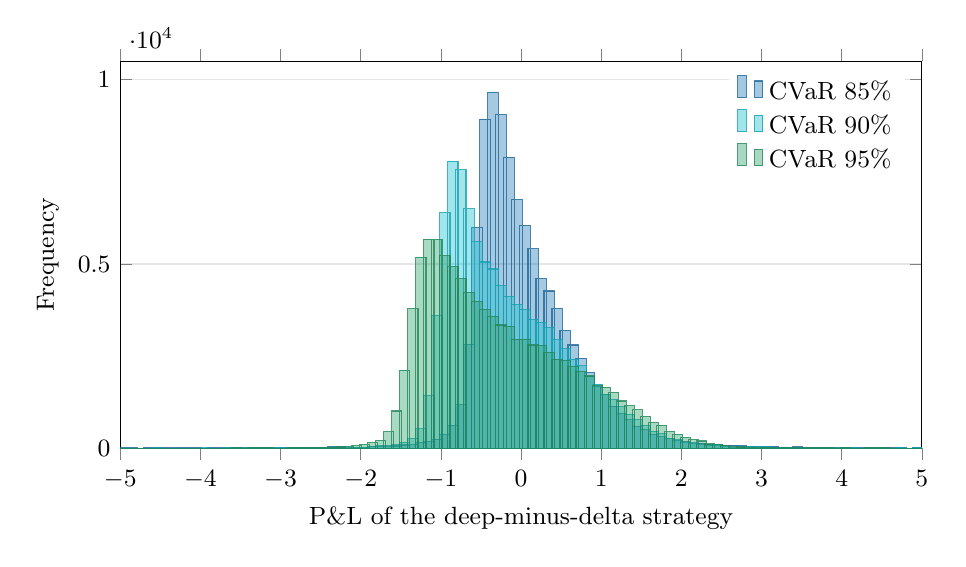
\begin{tikzpicture}
\begin{axis}[width=.97\linewidth,height=6.5cm,
 xlabel={P\&L of the deep-minus-delta strategy},ylabel={Frequency},
 xmin=-5,xmax=5,ymin=0,ymax=10500,
 ybar,bar shift=0pt,bar width=3.7pt,
 tick label style={font=\small},label style={font=\small},
 legend style={font=\small,draw=none,at={(.98,.98)},anchor=north east},
 ymajorgrids=true,grid style={black!10}]
\addplot[fill=panelblue,draw=panelblue!85!black,fill opacity=.4,draw opacity=.8,bar shift=0pt] coordinates {
(-4.95,13)
(-4.85,12)
(-4.75,7)
(-4.65,21)
(-4.55,10)
(-4.45,15)
(-4.35,10)
(-4.25,13)
(-4.15,19)
(-4.05,12)
(-3.95,9)
(-3.85,11)
(-3.75,14)
(-3.65,10)
(-3.55,17)
(-3.45,19)
(-3.35,20)
(-3.25,21)
(-3.15,16)
(-3.05,26)
(-2.95,22)
(-2.85,28)
(-2.75,23)
(-2.65,24)
(-2.55,33)
(-2.45,24)
(-2.35,38)
(-2.25,38)
(-2.15,29)
(-2.05,35)
(-1.95,34)
(-1.85,42)
(-1.75,45)
(-1.65,54)
(-1.55,66)
(-1.45,92)
(-1.35,98)
(-1.25,161)
(-1.15,183)
(-1.05,244)
(-0.95,370)
(-0.85,630)
(-0.75,1182)
(-0.65,2816)
(-0.55,5995)
(-0.45,8925)
(-0.35,9651)
(-0.25,9044)
(-0.15,7896)
(-0.05,6751)
(0.05,6045)
(0.15,5411)
(0.25,4611)
(0.35,4267)
(0.45,3793)
(0.55,3203)
(0.65,2804)
(0.75,2448)
(0.85,2062)
(0.95,1687)
(1.05,1468)
(1.15,1146)
(1.25,939)
(1.35,774)
(1.45,583)
(1.55,510)
(1.65,376)
(1.75,313)
(1.85,270)
(1.95,217)
(2.05,177)
(2.15,125)
(2.25,143)
(2.35,113)
(2.45,97)
(2.55,90)
(2.65,86)
(2.75,64)
(2.85,57)
(2.95,62)
(3.05,49)
(3.15,54)
(3.25,34)
(3.35,34)
(3.45,40)
(3.55,32)
(3.65,34)
(3.75,20)
(3.85,22)
(3.95,18)
(4.05,16)
(4.15,21)
(4.25,17)
(4.35,16)
(4.45,12)
(4.55,11)
(4.65,17)
(4.75,12)
(4.85,6)
(4.95,14)
};
\addlegendentry{CVaR 85\%}
\addplot[fill=panelcyan,draw=panelcyan!85!black,fill opacity=.4,draw opacity=.8,bar shift=0pt] coordinates {
(-4.95,6)
(-4.85,7)
(-4.75,3)
(-4.65,4)
(-4.55,11)
(-4.45,8)
(-4.35,7)
(-4.25,7)
(-4.15,4)
(-4.05,8)
(-3.95,13)
(-3.85,4)
(-3.75,7)
(-3.65,12)
(-3.55,10)
(-3.45,11)
(-3.35,12)
(-3.25,11)
(-3.15,19)
(-3.05,17)
(-2.95,21)
(-2.85,13)
(-2.75,17)
(-2.65,16)
(-2.55,18)
(-2.45,25)
(-2.35,21)
(-2.25,25)
(-2.15,30)
(-2.05,35)
(-1.95,33)
(-1.85,46)
(-1.75,74)
(-1.65,87)
(-1.55,101)
(-1.45,162)
(-1.35,269)
(-1.25,528)
(-1.15,1429)
(-1.05,3608)
(-0.95,6393)
(-0.85,7786)
(-0.75,7558)
(-0.65,6495)
(-0.55,5603)
(-0.45,5054)
(-0.35,4863)
(-0.25,4406)
(-0.15,4127)
(-0.05,3909)
(0.05,3769)
(0.15,3491)
(0.25,3423)
(0.35,3267)
(0.45,2944)
(0.55,2701)
(0.65,2418)
(0.75,2241)
(0.85,1947)
(0.95,1743)
(1.05,1464)
(1.15,1317)
(1.25,1125)
(1.35,926)
(1.45,775)
(1.55,622)
(1.65,467)
(1.75,394)
(1.85,279)
(1.95,234)
(2.05,157)
(2.15,151)
(2.25,113)
(2.35,82)
(2.45,91)
(2.55,48)
(2.65,34)
(2.75,36)
(2.85,57)
(2.95,41)
(3.05,38)
(3.15,35)
(3.25,30)
(3.35,23)
(3.45,15)
(3.55,17)
(3.65,18)
(3.75,16)
(3.85,17)
(3.95,13)
(4.05,8)
(4.15,17)
(4.25,7)
(4.35,9)
(4.45,18)
(4.55,9)
(4.65,7)
(4.75,11)
(4.85,7)
(4.95,11)
};
\addlegendentry{CVaR 90\%}
\addplot[fill=plotgreen,draw=plotgreen!85!black,fill opacity=.4,draw opacity=.8,bar shift=0pt] coordinates {
(-4.95,4)
(-4.85,5)
(-4.75,3)
(-4.65,4)
(-4.55,3)
(-4.45,4)
(-4.35,5)
(-4.25,7)
(-4.15,4)
(-4.05,4)
(-3.95,4)
(-3.85,8)
(-3.75,7)
(-3.65,8)
(-3.55,12)
(-3.45,8)
(-3.35,13)
(-3.25,15)
(-3.15,14)
(-3.05,4)
(-2.95,7)
(-2.85,15)
(-2.75,21)
(-2.65,14)
(-2.55,26)
(-2.45,30)
(-2.35,34)
(-2.25,39)
(-2.15,55)
(-2.05,72)
(-1.95,104)
(-1.85,153)
(-1.75,217)
(-1.65,449)
(-1.55,1015)
(-1.45,2123)
(-1.35,3787)
(-1.25,5182)
(-1.15,5673)
(-1.05,5668)
(-0.95,5224)
(-0.85,4923)
(-0.75,4596)
(-0.65,4227)
(-0.55,3988)
(-0.45,3771)
(-0.35,3586)
(-0.25,3347)
(-0.15,3310)
(-0.05,2961)
(0.05,2959)
(0.15,2804)
(0.25,2784)
(0.35,2601)
(0.45,2421)
(0.55,2372)
(0.65,2212)
(0.75,2084)
(0.85,1963)
(0.95,1710)
(1.05,1658)
(1.15,1518)
(1.25,1284)
(1.35,1160)
(1.45,1045)
(1.55,869)
(1.65,704)
(1.75,630)
(1.85,456)
(1.95,385)
(2.05,289)
(2.15,236)
(2.25,201)
(2.35,118)
(2.45,100)
(2.55,71)
(2.65,43)
(2.75,38)
(2.85,35)
(2.95,29)
(3.05,21)
(3.15,20)
(3.25,14)
(3.35,11)
(3.45,14)
(3.55,13)
(3.65,12)
(3.75,13)
(3.85,16)
(3.95,5)
(4.05,19)
(4.15,5)
(4.25,8)
(4.35,10)
(4.45,10)
(4.55,12)
(4.65,5)
(4.75,7)
(4.85,8)
(4.95,1)
};
\addlegendentry{CVaR 95\%}
\end{axis}
\end{tikzpicture}
\caption{Independent reproduction of Figure 1, Panel B: zero-capital difference-strategy profits for the 85\%, 90\% and 95\% agents. All base hedges start at 3.16. Common bins have width 0.1; outcomes outside the displayed range remain in all statistics.}
\label{fig:panelb}
\end{figure}
The numbers outside $[-5,5]$ are 85\%: 712, 90\%: 384, 95\%: 244. All outcomes are retained in the supplied terminal arrays. The independent curves and statistics do not exactly reproduce the published experiment.

\subsection{Standalone hedge distributions and centring}

I extract the standalone outcomes from the same 100,000 physical test paths used for Panel B, with initial capital 3.16. For a short call, terminal net profit is hedge wealth after settling the payoff:
\begin{align*}
 \Pi_T^{(a)}&=V_T^{\rm DH,(a)}-H=-L^{\rm DH,(a)},
 &\Pi_T^\Delta&=V_T^\Delta-H=-L^\Delta,\\
 \Pi_T^{(a)}-\Pi_T^\Delta
 &=V_T^{\rm DH,(a)}-H-V_T^\Delta+H
 =V_T^{\rm DH,(a)}-V_T^\Delta=U_T^{(a)}.
\end{align*}
These are the complete hedged short-call positions. I retain their original sign and location; loss distributions are their reflections about zero.

For observations $p_1,\ldots,p_n$, I calculate $\overline p=n^{-1}\sum_i p_i$. Order them as $p_{(1)}\leq\cdots\leq p_{(n)}$. For quantile level $b$, let $z=(n-1)b$, $j=\lfloor z\rfloor$ and $w=z-j$. Linear interpolation gives
\[
 \widehat q_b=(1-w)p_{(j+1)}+wp_{(\min(j+2,n))}.
\]
The median is consequently $(p_{(50,000)}+p_{(50,001)})/2$. The negative-profit fraction is $n^{-1}\sum_i\mathbf1_{\{p_i<0\}}$.

\begin{table}[htbp]
\centering\small
\caption{Standalone net profit on the common physical test sample. All 100,000 outcomes enter each statistic.}
\begin{tabular}{@{}lrrrrr@{}}
\toprule
Hedge & Mean & Median & 5th percentile & 95th percentile & Negative profit\\
\midrule
Deep (85\%) & 0.666066 & 0.785888 & -0.770513 & 2.159817 & 13.913\% \\
Deep (90\%) & 0.488881 & 0.514722 & -0.992383 & 2.167698 & 26.009\% \\
Deep (95\%) & 0.388896 & 0.399363 & -1.412509 & 2.251163 & 34.652\% \\
Delta & 0.651676 & 0.971850 & -1.406855 & 1.690658 & 17.489\% \\
\bottomrule
\end{tabular}
\end{table}

All four sample means and medians are positive; none is centred at zero. The distributions are asymmetric. For the 95\% agent, the sample identity is
\[
 \overline\Pi_T^{(.95)}-\overline\Pi_T^\Delta
 =0.388896465-0.651675992=-0.262779527
 =\overline U_T^{(.95)}.
\]
The pathwise identity holds within $1.8\times10^{-15}$. All saved outcomes are finite. The observed standalone ranges are $[-61.256421,20.552935]$, $[-58.352098,19.954393]$, $[-57.973946,12.486723]$ and $[-38.283843,2.484203]$ for the three deep hedges and delta. These are sample ranges, not bounds on possible outcomes.

For edges $b_j=-5+0.1j$, I count $N_j=\sum_i\mathbf1_{\{b_{j-1}\leq p_i<b_j\}}$, including the last upper endpoint. The histogram height is $N_j/(100,000\times0.1)$. Its central area is the fraction within the displayed range. The respective counts outside $[-5,5]$ are 945, 618, 534 and 527. All observations remain in the numerical summaries and complete empirical distributions.
\begin{figure}[htbp]
\centering
% Author: Amanjeet Singh
% Requires tikz and pgfplots.
\definecolor{standDeepA}{HTML}{1F77B4}
\definecolor{standDeepB}{HTML}{17BECF}
\definecolor{standDeepC}{HTML}{279E68}
\definecolor{standDelta}{HTML}{D97925}
\begin{tikzpicture}
\begin{axis}[name=standdeep,width=.475\linewidth,height=5.4cm,xmin=-5,xmax=5,ymin=0,ymax=0.84896,xlabel={Terminal net hedge P\&L},grid=major,grid style={gray!15},tick label style={font=\scriptsize},label style={font=\small},title style={font=\small},legend style={font=\scriptsize,draw=none,fill=none,at={(0.02,0.98)},anchor=north west},title={Deep hedges},ylabel={Full-sample empirical density}]
\addplot[const plot,no marks,color=standDeepA,line width=.9pt] coordinates {(-5,0.0024) (-4.9,0.0021) (-4.8,0.0019) (-4.7,0.0032) (-4.6,0.0028) (-4.5,0.003) (-4.4,0.0031) (-4.3,0.0028) (-4.2,0.0029) (-4.1,0.0034) (-4,0.0032) (-3.9,0.003) (-3.8,0.0038) (-3.7,0.005) (-3.6,0.003) (-3.5,0.0047) (-3.4,0.005) (-3.3,0.0059) (-3.2,0.0051) (-3.1,0.0048) (-3,0.0064) (-2.9,0.0058) (-2.8,0.0085) (-2.7,0.0055) (-2.6,0.0076) (-2.5,0.008) (-2.4,0.0101) (-2.3,0.0087) (-2.2,0.01) (-2.1,0.0103) (-2,0.0116) (-1.9,0.0131) (-1.8,0.0142) (-1.7,0.0136) (-1.6,0.0149) (-1.5,0.015) (-1.4,0.0236) (-1.3,0.0213) (-1.2,0.0216) (-1.1,0.028) (-1,0.0302) (-0.9,0.0353) (-0.8,0.0429) (-0.7,0.0438) (-0.6,0.0601) (-0.5,0.0717) (-0.4,0.0852) (-0.3,0.1191) (-0.2,0.1824) (-0.1,0.2978) (0,0.4684) (0.1,0.3285) (0.2,0.321) (0.3,0.3855) (0.4,0.4668) (0.5,0.5351) (0.6,0.5924) (0.7,0.5956) (0.8,0.5832) (0.9,0.542) (1,0.4736) (1.1,0.4282) (1.2,0.3925) (1.3,0.3544) (1.4,0.3201) (1.5,0.28) (1.6,0.2476) (1.7,0.2196) (1.8,0.1872) (1.9,0.1618) (2,0.1491) (2.1,0.1209) (2.2,0.0973) (2.3,0.0866) (2.4,0.0709) (2.5,0.0509) (2.6,0.0438) (2.7,0.0326) (2.8,0.0243) (2.9,0.0154) (3,0.0112) (3.1,0.0076) (3.2,0.0052) (3.3,0.0033) (3.4,0.0015) (3.5,0.001) (3.6,0.001) (3.7,0.0004) (3.8,0.0001) (3.9,0.0004) (4,0.0002) (4.1,0.0001) (4.2,0) (4.3,0.0002) (4.4,0.0002) (4.5,0.0001) (4.6,0) (4.7,0.0003) (4.8,0) (4.9,0) (5,0)};
\addlegendentry{CVaR 85\%}
\addplot[forget plot,no marks,dashed,color=standDeepA,line width=.55pt] coordinates {(0.6660658344,0) (0.6660658344,0.84896)};
\addplot[const plot,no marks,color=standDeepB,line width=.9pt] coordinates {(-5,0.0024) (-4.9,0.0017) (-4.8,0.0017) (-4.7,0.0017) (-4.6,0.0025) (-4.5,0.0025) (-4.4,0.0033) (-4.3,0.003) (-4.2,0.0017) (-4.1,0.003) (-4,0.0022) (-3.9,0.0033) (-3.8,0.0032) (-3.7,0.0044) (-3.6,0.0032) (-3.5,0.0048) (-3.4,0.0046) (-3.3,0.0053) (-3.2,0.0058) (-3.1,0.007) (-3,0.0068) (-2.9,0.0076) (-2.8,0.0081) (-2.7,0.0079) (-2.6,0.0086) (-2.5,0.0101) (-2.4,0.0109) (-2.3,0.011) (-2.2,0.0132) (-2.1,0.0154) (-2,0.0157) (-1.9,0.0169) (-1.8,0.0169) (-1.7,0.0187) (-1.6,0.0245) (-1.5,0.0246) (-1.4,0.0288) (-1.3,0.0331) (-1.2,0.0448) (-1.1,0.0438) (-1,0.0612) (-0.9,0.0812) (-0.8,0.1374) (-0.7,0.2477) (-0.6,0.2672) (-0.5,0.2161) (-0.4,0.2149) (-0.3,0.2315) (-0.2,0.294) (-0.1,0.3542) (0,0.4255) (0.1,0.4774) (0.2,0.4756) (0.3,0.4785) (0.4,0.474) (0.5,0.4311) (0.6,0.4034) (0.7,0.3743) (0.8,0.3649) (0.9,0.3429) (1,0.3112) (1.1,0.3031) (1.2,0.2848) (1.3,0.2763) (1.4,0.2449) (1.5,0.2368) (1.6,0.2169) (1.7,0.2012) (1.8,0.1803) (1.9,0.1657) (2,0.1383) (2.1,0.1335) (2.2,0.1092) (2.3,0.0922) (2.4,0.0723) (2.5,0.0587) (2.6,0.0425) (2.7,0.0325) (2.8,0.0221) (2.9,0.0127) (3,0.0068) (3.1,0.0045) (3.2,0.0016) (3.3,0.0011) (3.4,0.0003) (3.5,0) (3.6,0.0002) (3.7,0.0003) (3.8,0.0001) (3.9,0.0001) (4,0.0001) (4.1,0.0001) (4.2,0.0001) (4.3,0) (4.4,0) (4.5,0) (4.6,0) (4.7,0) (4.8,0) (4.9,0) (5,0)};
\addlegendentry{CVaR 90\%}
\addplot[forget plot,no marks,dashed,color=standDeepB,line width=.55pt] coordinates {(0.4888806736,0) (0.4888806736,0.84896)};
\addplot[const plot,no marks,color=standDeepC,line width=.9pt] coordinates {(-5,0.0016) (-4.9,0.0017) (-4.8,0.0014) (-4.7,0.0024) (-4.6,0.002) (-4.5,0.0019) (-4.4,0.0017) (-4.3,0.0025) (-4.2,0.0035) (-4.1,0.0022) (-4,0.0036) (-3.9,0.004) (-3.8,0.0037) (-3.7,0.0052) (-3.6,0.0027) (-3.5,0.0028) (-3.4,0.0047) (-3.3,0.0053) (-3.2,0.0064) (-3.1,0.0069) (-3,0.0059) (-2.9,0.008) (-2.8,0.0085) (-2.7,0.0082) (-2.6,0.0109) (-2.5,0.0116) (-2.4,0.0117) (-2.3,0.0144) (-2.2,0.0159) (-2.1,0.0186) (-2,0.0196) (-1.9,0.0237) (-1.8,0.034) (-1.7,0.0448) (-1.6,0.0601) (-1.5,0.0982) (-1.4,0.1327) (-1.3,0.1154) (-1.2,0.1057) (-1.1,0.1095) (-1,0.1151) (-0.9,0.1332) (-0.8,0.1461) (-0.7,0.1792) (-0.6,0.2078) (-0.5,0.2594) (-0.4,0.3321) (-0.3,0.3516) (-0.2,0.3824) (-0.1,0.382) (0,0.3848) (0.1,0.4009) (0.2,0.3852) (0.3,0.3667) (0.4,0.3506) (0.5,0.3381) (0.6,0.3306) (0.7,0.3303) (0.8,0.2953) (0.9,0.2941) (1,0.2705) (1.1,0.2652) (1.2,0.2574) (1.3,0.2374) (1.4,0.223) (1.5,0.2142) (1.6,0.2068) (1.7,0.1924) (1.8,0.1767) (1.9,0.1619) (2,0.1481) (2.1,0.141) (2.2,0.1233) (2.3,0.1026) (2.4,0.0935) (2.5,0.073) (2.6,0.0581) (2.7,0.0417) (2.8,0.0316) (2.9,0.0191) (3,0.0113) (3.1,0.0046) (3.2,0.0021) (3.3,0.0006) (3.4,0.0005) (3.5,0) (3.6,0.0001) (3.7,0.0001) (3.8,0.0002) (3.9,0.0001) (4,0.0001) (4.1,0) (4.2,0) (4.3,0) (4.4,0) (4.5,0.0001) (4.6,0.0002) (4.7,0) (4.8,0) (4.9,0) (5,0)};
\addlegendentry{CVaR 95\%}
\addplot[forget plot,no marks,dashed,color=standDeepC,line width=.55pt] coordinates {(0.388896465,0) (0.388896465,0.84896)};
\addplot[forget plot,no marks,black,line width=.6pt] coordinates {(0,0) (0,0.84896)};
\end{axis}
\begin{axis}[name=standdelta,width=.475\linewidth,height=5.4cm,xmin=-5,xmax=5,ymin=0,ymax=0.84896,xlabel={Terminal net hedge P\&L},grid=major,grid style={gray!15},tick label style={font=\scriptsize},label style={font=\small},title style={font=\small},legend style={font=\scriptsize,draw=none,fill=none,at={(0.02,0.98)},anchor=north west},title={Common delta hedge},at={(standdeep.east)},anchor=west,xshift=.03\linewidth,yticklabels={}]
\addplot[const plot,no marks,color=standDelta,line width=.9pt] coordinates {(-5,0.0025) (-4.9,0.0025) (-4.8,0.0027) (-4.7,0.0026) (-4.6,0.0029) (-4.5,0.0034) (-4.4,0.0034) (-4.3,0.0042) (-4.2,0.0044) (-4.1,0.0053) (-4,0.0045) (-3.9,0.0053) (-3.8,0.0056) (-3.7,0.0077) (-3.6,0.0078) (-3.5,0.0063) (-3.4,0.0069) (-3.3,0.01) (-3.2,0.008) (-3.1,0.0122) (-3,0.0121) (-2.9,0.0112) (-2.8,0.0126) (-2.7,0.0132) (-2.6,0.0178) (-2.5,0.0153) (-2.4,0.0168) (-2.3,0.0204) (-2.2,0.0199) (-2.1,0.0202) (-2,0.0223) (-1.9,0.0293) (-1.8,0.0265) (-1.7,0.0313) (-1.6,0.0342) (-1.5,0.0381) (-1.4,0.043) (-1.3,0.0472) (-1.2,0.0546) (-1.1,0.0555) (-1,0.065) (-0.9,0.0706) (-0.8,0.0799) (-0.7,0.0831) (-0.6,0.094) (-0.5,0.1056) (-0.4,0.1151) (-0.3,0.1247) (-0.2,0.1453) (-0.1,0.1632) (0,0.1794) (0.1,0.1989) (0.2,0.2274) (0.3,0.2559) (0.4,0.2893) (0.5,0.3382) (0.6,0.3765) (0.7,0.4472) (0.8,0.518) (0.9,0.595) (1,0.6824) (1.1,0.7517) (1.2,0.758) (1.3,0.6915) (1.4,0.6259) (1.5,0.4858) (1.6,0.3591) (1.7,0.2181) (1.8,0.1277) (1.9,0.0698) (2,0.032) (2.1,0.0131) (2.2,0.0072) (2.3,0.0022) (2.4,0.0008) (2.5,0) (2.6,0) (2.7,0) (2.8,0) (2.9,0) (3,0) (3.1,0) (3.2,0) (3.3,0) (3.4,0) (3.5,0) (3.6,0) (3.7,0) (3.8,0) (3.9,0) (4,0) (4.1,0) (4.2,0) (4.3,0) (4.4,0) (4.5,0) (4.6,0) (4.7,0) (4.8,0) (4.9,0) (5,0)};
\addlegendentry{Delta hedge}
\addplot[forget plot,no marks,dashed,color=standDelta,line width=.55pt] coordinates {(0.651675992,0) (0.651675992,0.84896)};
\addplot[forget plot,no marks,black,line width=.6pt] coordinates {(0,0) (0,0.84896)};
\end{axis}
\end{tikzpicture}
% Density=count/(100000*bin width); unchanged net P&L; S0=100 and initial capital 3.16.
\caption{Standalone short-call hedging profits at their original locations. The black lines mark zero and dashed lines mark sample means. Common bins of width 0.1 use the full-sample denominator.}
\label{fig:standalone}
\end{figure}

Zero mean is not a defining property of a hedge evaluated under the physical measure. To distinguish this from pricing, suppose the wealth and predictable trading gains are integrable under the selected measure $\mathbb Q$. Then
\begin{align*}
 \mathbb E_{\mathbb Q}[V_{t+1}\mid\mathcal F_t]
 &=e^{r\Delta t}V_t+\delta_t\bigl(e^{q\Delta t}
     \mathbb E_{\mathbb Q}[S_{t+1}\mid\mathcal F_t]
                 -e^{r\Delta t}S_t\bigr)\\
 &=e^{r\Delta t}V_t+\delta_t\bigl(e^{q\Delta t}
       S_te^{(r-q)\Delta t}-e^{r\Delta t}S_t\bigr)
 =e^{r\Delta t}V_t.
\end{align*}
Iterating the tower property and using the pricing definition gives
\begin{align*}
 \mathbb E_{\mathbb Q}[V_{t+1}]
 &=\mathbb E_{\mathbb Q}\!\left[\mathbb E_{\mathbb Q}[V_{t+1}\mid\mathcal F_t]\right]
 =e^{r\Delta t}\mathbb E_{\mathbb Q}[V_t],\\
 \mathbb E_{\mathbb Q}[V_T]&=e^{r\Delta t}\mathbb E_{\mathbb Q}[V_{T-1}]
 =\cdots=e^{rT\Delta t}V_0,
 &C_0&=e^{-rT\Delta t}\mathbb E_{\mathbb Q}[H],\\
 \mathbb E_{\mathbb Q}[\Pi_T]
 &=\mathbb E_{\mathbb Q}[V_T]-\mathbb E_{\mathbb Q}[H]
 =e^{rT\Delta t}(V_0-C_0).
\end{align*}
This identity requires integrability and concerns $\mathbb Q$; the histograms use $\mathbb P$. It supplies no zero-centre requirement for these physical samples. Training minimises upper-tail loss rather than imposing a mean constraint.

Under $\mathbb P$, the conditional normal moment instead gives
\begin{align*}
 \mathbb E_{\mathbb P}[S_{t+1}\mid\mathcal F_t]
 &=S_te^\mu\mathbb E[e^{\sqrt{h_t}\varepsilon_{t+1}}]
 =S_te^{\mu+h_t/2},\\
 \mathbb E_{\mathbb P}[g_t\mid\mathcal F_t]
 &=S_t\bigl(e^{q\Delta t+\mu+h_t/2}-e^{r\Delta t}\bigr).
\end{align*}
This conditional stock gain is positive for the retained parameters because $\mu+h_t/2>(r-q)\Delta t$. It does not determine the unconditional profit of a hedged call.

The deterministic capital excess relative to the estimated model price is
\[
 e^{rT\Delta t}(3.16-2.770068435)=0.391562932.
\]
It is common to both hedges and cancels from their difference when positions are fixed. It is not an estimate of their physical expected profit. The fixed-position translation at the lower capital breaches the neural borrowing limit, as shown above. Population centring and normal-approximation coverage also require the hedge-loss moment conditions discussed in this note.

\subsection{Calibration and initial variance}
I investigate the initial variance and numerical calibration while keeping initial capital 3.16, the 95\% objective, architecture and seeds fixed. The two new policies complete 50 epochs on 400,000 training and 50,000 validation paths. Validation selects epoch 47 for the larger initial state and epoch 50 for the percentage-unit fit. All comparisons use 100,000 test paths with the same innovations as the retained baseline. Each market has its own conditional delta benchmark.

The observed final return is $r_n=0.006418204633$. Its fitted residual and next-return variance follow directly from the GJR recursion:
\begin{align}
 u_n&=r_n-\mu=0.005792913946>0,\nonumber\\
 h_{\rm next}&=\omega+(\alpha+\gamma\mathbf1_{\{u_n<0\}})u_n^2+\beta h_n\nonumber\\
 &=\omega+\alpha u_n^2+\beta h_n
 =2.666633546772747\times10^{-5}.
\end{align}
This is 2.236\% above the retained terminal fitted variance. I re-evaluate the baseline weights under this initial-state change. The price-compatible state $7.75\times10^{-5}$ was fixed by the earlier option-price comparison; I retrain its policy. I also retrain using the previously recorded percentage-unit likelihood fit. These choices precede the new hedging-loss evaluations.

\begin{table}[htbp]
\centering\footnotesize
\caption{Calibration sensitivities at confidence 0.95. Capital is 3.16 throughout. The forecast row uses the baseline weights; the other two controls use separately retrained policies. Prices use seed 46; independent seed-47 checks are retained.}
\begin{tabular}{@{}lrrrrrr@{}}
\toprule
Setup & Price & DH CVaR & Delta CVaR & Gap & Overlay CVaR & Mean profit\\
\midrule
Published & 3.160 & 3.481 & 3.562 & -0.081 & 1.810 & -0.254\\
Baseline & 2.770068 & 2.884726 & 2.959946 & -0.075220 & 1.865054 & -0.262780\\
Forecast & 2.775015 & 2.900073 & 2.973967 & -0.073895 & 1.869286 & -0.262345\\
Price-compatible state & 3.160828 & 4.010514 & 4.125525 & -0.115011 & 2.329686 & -0.168131\\
Scaled fit & 3.052934 & 4.353688 & 4.429238 & -0.075551 & 2.131629 & -0.268979\\
\bottomrule
\end{tabular}
\end{table}
\begin{figure}[htbp]
\centering
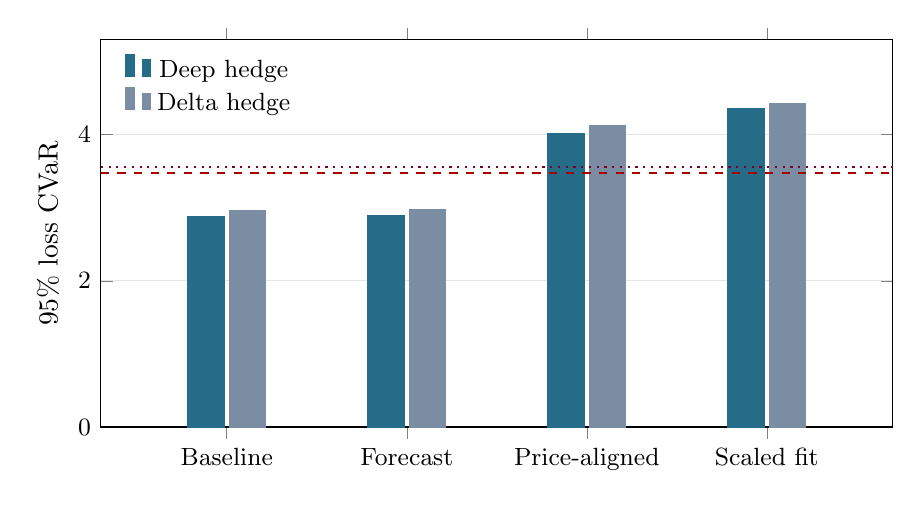
\begin{tikzpicture}
\begin{axis}[width=.96\linewidth,height=6.5cm,ybar,bar width=13pt,
 ymin=0,ymax=5.3,xmin=-.7,xmax=3.7,
 xtick={0,1,2,3},xticklabels={Baseline,Forecast,Price-aligned,Scaled fit},
 ylabel={95\% loss CVaR},legend style={draw=none,font=\small,at={(.02,.98)},anchor=north west},
 tick label style={font=\small},ymajorgrids=true,grid style={black!10}]
\addplot[fill=plotblue,draw=plotblue] coordinates {(0,2.884725659)(1,2.900072669)(2,4.010514281)(3,4.353687513)};
\addlegendentry{Deep hedge}
\addplot[fill=plotslate,draw=plotslate] coordinates {(0,2.959945763)(1,2.973967205)(2,4.125525449)(3,4.429238282)};
\addlegendentry{Delta hedge}
\draw[red!65!black,dashed,thick] (axis cs:-.7,3.481)--(axis cs:3.7,3.481);
\draw[purple!65!black,dotted,thick] (axis cs:-.7,3.562)--(axis cs:3.7,3.562);
\end{axis}
\end{tikzpicture}
\caption{Calibration controls at capital 3.16. The forecast uses baseline weights; the two larger controls are retrained. Horizontal lines mark the published deep CVaR 3.481 and implied delta CVaR 3.562. These are empirical point estimates.}
\label{fig:calibrationrisk}
\end{figure}
The forecasting convention changes the call value by about 0.005 and deep-hedging CVaR by 0.015347. The larger initial state prices the call near 3.16, but its retrained CVaR is 4.010514; the scaled-fit control gives 4.353688. Neither reproduces the published 3.481.

To separate a change of market inputs from a change of weights, let $\rho_s(\theta)$ denote empirical 95\% loss CVaR for policy weights $\theta$ in scenario $s$. Write $\theta_0$ for the retained policy and $\theta_s$ for its retrained counterpart. Adding and subtracting the same quantity gives
\begin{align}
 \rho_s(\theta_s)-\rho_0(\theta_0)
 &=\rho_s(\theta_s)-\rho_s(\theta_0)
   +\rho_s(\theta_0)-\rho_0(\theta_0)\nonumber\\
 &=B_s+A_s,\nonumber\\
 A_s&=\rho_s(\theta_0)-\rho_0(\theta_0),\qquad
 B_s=\rho_s(\theta_s)-\rho_s(\theta_0).
\end{align}
For the price-compatible state, $A_s=1.351115$, $B_s=-0.225326$, and the total change is 1.125789. For the scaled fit, the corresponding values are 1.570174, $-0.101212$ and 1.468962. Fixed weights still produce different positions because the market and evolving wealth inputs change. Most of the standalone-risk increase is present before retraining; retraining reduces it. This decomposition describes the controlled simulations and does not identify the original published calibration.

\begin{table}[htbp]
\centering\small
\caption{Independent price diagnostics, each using two million paths and the bounded conditional-put estimator. The last two rows are explicitly hybrid unit and coefficient checks.}
\begin{tabular}{@{}lrr@{}}
\toprule
Input convention & Seed 46 & Seed 47\\
\midrule
Retained fitted state & 2.770068 & 2.770844\\
Observed-residual forecast & 2.775015 & 2.775785\\
Price-compatible initial state & 3.160828 & 3.161292\\
Percentage-unit fit & 3.052934 & 3.054692\\
Printed coefficients, retained intercept & 2.977228 & 2.978517\\
Literal daily intercept $0.0001$ & 14.383069 & 14.392754\\
\bottomrule
\end{tabular}
\end{table}
The literal-intercept price is about 14.38. This tests one possible reading of the printed percentage, rather than establishing the paper's intended variance units. The hybrid coefficient check retains the fitted intercept and initial state while replacing only the printed mean, ARCH, leverage and GARCH coefficients.

The five percentage-unit starts give log likelihood 4300.789537361 in decimal units. Their spread is below $4.3\times10^{-11}$. This is within $2.8\times10^{-8}$ of the earlier scaled fit and above the raw fit's 4298.041204605. I retain the predefined inputs for the sensitivity runs. Agreement of these starts supports numerical consistency without proving a global maximum or recovering the original fit.

\subsubsection{Physical variance moments}
Write $A(Z)=\beta+(\alpha+\gamma\mathbf1_{\{Z<0\}})Z^2$, so $h_{t+1}=\omega+A(Z_{t+1})h_t$. Standard-normal symmetry gives $\mathbb E[Z^2]=1$ and $\mathbb E[Z^2\mathbf1_{\{Z<0\}}]=1/2$. Since $\varphi'(z)=-z\varphi(z)$, integration by parts gives
\[
 \mathbb E[Z^4]=-\int_{\mathbb R}z^3\varphi'(z)\,dz
 =3\int_{\mathbb R}z^2\varphi(z)\,dz=3,
 \qquad \mathbb E[Z^4\mathbf1_{\{Z<0\}}]=\frac32.
\]
The Gaussian boundary term vanishes. Expanding the first two moments of $A$ yields
\begin{align}
 \psi:=\mathbb E[A]&=\beta+\alpha+\gamma/2,\nonumber\\
 \chi:=\mathbb E[A^2]
 &=\beta^2+2\beta\,\mathbb E[(\alpha+\gamma\mathbf1_{\{Z<0\}})Z^2]
   +\mathbb E[(\alpha+\gamma\mathbf1_{\{Z<0\}})^2Z^4]\nonumber\\
 &=\beta^2+2\beta(\alpha+\gamma/2)
   +3\alpha^2+\tfrac32(2\alpha\gamma+\gamma^2).
\end{align}
Let $m_t=\mathbb E_{\Pp}[h_t]$ and $s_t=\mathbb E_{\Pp}[h_t^2]$. Independence of the next innovation and known current variance gives
\begin{align}
 m_{t+1}&=\omega+\psi m_t,\qquad m_0=h_0,\nonumber\\
 s_{t+1}&=\mathbb E[\omega^2+2\omega A h_t+A^2h_t^2]
          =\omega^2+2\omega\psi m_t+\chi s_t,
          \qquad s_0=h_0^2.
\end{align}
Unrolling the first recursion and summing its geometric series gives
\begin{align}
 m_t&=\psi^t h_0+\omega\sum_{j=0}^{t-1}\psi^j
     =\psi^t h_0+\frac{\omega(1-\psi^t)}{1-\psi}\nonumber\\
 &=\bar h+\psi^t(h_0-\bar h),\qquad \bar h=\frac{\omega}{1-\psi},\nonumber\\
 \frac1T\sum_{t=0}^{T-1}m_t
 &=\bar h+(h_0-\bar h)\frac{1-\psi^T}{T(1-\psi)}.
\end{align}
With identical coefficients, changing only the initial variance gives $m_t'-m_t=\psi^t(h_0'-h_0)$. Thus the larger initial state affects variance throughout the horizon. Conditional Gaussianity also gives
\[
 \mathbb E_{\Pp}[(R_{t+1}-\mu)^4]
 =\mathbb E[h_t^2\,\mathbb E[Z_{t+1}^4\mid\F_t]]=3s_t.
\]
The physical annualised RMS volatility is $\sqrt{252T^{-1}\sum_{t=0}^{T-1}m_t}$. It is 14.0613\% for the baseline, 14.0911\% for the observed forecast, 16.4850\% for the larger state and 16.1306\% for the scaled fit. The baseline has $(\psi,\chi)=(0.979999777,1.070399523)$; the scaled fit has $(0.983436482,1.145044007)$. Their mean-variance persistence is similar, while the second-moment recursion differs substantially.

All finite-date moments in these recursions are finite. If a stationary second variance moment were finite, it would satisfy $(1-\chi)s=\omega^2+2\omega\psi\bar h>0$, requiring $\chi<1$. Neither coefficient set satisfies that condition. This does not establish hedge-loss moments; the qualification in Section~\ref{sec:moments} remains applicable. These physical variance quantities are distinct from the option prices calculated under $\Q$.

\subsubsection{Numerical checks and public source comparison}
The two new initial deltas are independently checked with 500,000 stock-measure paths and analytic final-day integration. Grid-minus-Monte-Carlo differences are 0.334 and 0.798 sampling standard errors for the larger initial state and scaled fit. These are initial-state diagnostics rather than global error bounds. All five evaluated policy rows retain finite terminal records and satisfy the borrowing test within its 0.001 tolerance. Accounting identity errors are below $5.7\times10^{-14}$, and the decomposition sums agree exactly.

The public repository also contains GJR aggregate results in \texttt{metrics.csv}: its 95\% row records option price 3.157065, deep-hedging CVaR 3.024906, overlay CVaR 1.979994 and mean profit $-0.307759$. These values differ from the published table. The aggregate file does not store the fitted coefficients, initial variance or model weights. The source additionally uses an artificial initial residual and a different saved volatility timing; that procedure is distinct from the observed-residual forecast above.

The nominal starting-capital check, forecast convention and two retraining controls do not reconcile the published standalone risk. The controls show that changing the market inputs moves both base risks together, while matching one option value leaves the joint path distribution and physical tail risk undetermined. A direct identification of the published run requires its full-precision calibration, initial state and trained policy.

\section{A moment qualification}\label{sec:moments}
\begin{proposition}[Infinite physical stock and call means]
For the retained physical model, $\alpha>0$, $h_0>0$, $\beta\geq0$, $\omega\geq0$ and $\alpha+\gamma\geq0$. At any horizon $T\geq3$,
\begin{equation}
 \E_{\Pp}[S_T]=\infty,\qquad\E_{\Pp}[(S_T-K)^+]=\infty.
\end{equation}
\end{proposition}
\begin{proof}
Let the first physical innovations be $z_1,z_2,z_3$. On $z_1,z_2>0$, the non-negative terms in \eqref{eq:physicalvariance} imply
\begin{equation}
 h_1\geq\alpha h_0z_1^2,\qquad
 h_2\geq\alpha h_1z_2^2\geq\alpha^2h_0z_1^2z_2^2.
\end{equation}
Integrating the third standard normal, conditional on $z_1,z_2$, gives
\begin{equation}
 \E_{\Pp}[S_3\mid z_1,z_2]
 =S_0\exp\!\left(3\mu+\sqrt{h_0}z_1+\sqrt{h_1}z_2+\frac{h_2}{2}\right).
 \label{eq:momentconditional}
\end{equation}
Choose $R>0$, restrict $z_1=x\geq R$ and $z_2\in[x,x+1]$, and integrate over this strip. The joint normal density is at least $(2\pi)^{-1}\exp(-x^2-x-1/2)$. The positive linear terms in \eqref{eq:momentconditional} may be discarded and $z_1^2z_2^2\geq x^4$. Tonelli's theorem applies to the non-negative stock, so
\begin{equation}
 \E_{\Pp}[S_3]\geq\frac{S_0e^{3\mu}}{2\pi}
       \int_R^\infty\exp\!\left(\frac{\alpha^2h_0}{2}x^4-x^2-x-\frac12\right)dx
       =\infty.
\end{equation}
For an explicit divergence comparison, set $A=\alpha^2h_0/2>0$. Since
$(x^2+x+1/2)/x^4\longrightarrow0$, there is $R_1\geq R$ such that
$x^2+x+1/2\leq Ax^4/2$ for $x\geq R_1$. The integrand is then at least
$\exp(Ax^4/2)\geq1$, so its integral is at least
$\int_{R_1}^{\infty}1\,dx=\infty$.

For later dates, condition first on the known state and integrate its normal innovation:
\begin{align}
 \E_{\Pp}[S_{t+1}\mid\F_t]
 &=S_t e^\mu\,\E[e^{\sqrt{h_t}\varepsilon_{t+1}}\mid\F_t]\nonumber\\
 &=S_t e^{\mu+h_t/2}\geq e^\mu S_t.
\end{align}
The tower property is valid for these non-negative variables even when expectations are infinite. Thus
\begin{equation}
 \E_{\Pp}[S_{t+1}]
 =\E_{\Pp}[S_t e^{\mu+h_t/2}]
 \geq e^\mu\E_{\Pp}[S_t]=\infty
 \qquad\text{whenever }\E_{\Pp}[S_t]=\infty.
\end{equation}
Induction from $t=3$ proves the stock assertion for every $T\geq3$. Finally
$S_T\leq(S_T-K)^++K$ implies
\begin{equation}
 \infty=\E_{\Pp}[S_T]\leq\E_{\Pp}[(S_T-K)^+]+K,
\end{equation}
which is possible only if the call's expectation is infinite.
\end{proof}
\begin{remark}
This proof concerns the stock and standalone payoff under $\Pp$. It does not prove that hedging-loss or overlay moments are infinite: cancellation between the payoff and portfolio, or between two portfolios, must be analysed separately. Their required moments remain unresolved here. Finite realised paths and small empirical standard errors alone do not establish those moments. The pricing calculation is unaffected by this physical-payoff conclusion: under the selected $\Q$ the stock first moment is finite, and its estimator in \eqref{eq:priceestimator} uses bounded put observations.
\end{remark}

\section{Numerical verification and comparison}
\subsection{Numerical identities}
All 13 independent checks in \texttt{verification.json} pass. They compare \eqref{eq:wealth} with separately tracked cash and stock accounts for fixed long positions, short positions and a binding cap. They also test the constant-hedge analytical CVaR gradient, tail selection, the zero-capital identity, TorchScript agreement, seed reproducibility, the known initial variance and predictability when future observations are altered. The constant-hedge automatic gradient is $-3.399353027$, compared with $-3.399352816$ analytically. Cash-account discrepancies are below $4.8\times10^{-7}$.
\begin{table}[htbp]
\centering\small
\caption{Checks on the complete 100,000-path test sample. The cash discrepancies are within the declared 0.001 floating-point tolerance.}
\label{tab:identitychecks}
\begin{tabular}{@{}lr@{}}
\toprule
Check & Observed value\\\midrule
$\max_i|U_i-(V_i^{\rm DH}-V_i^\Delta)|$ & $4.2632564146\times 10^{-14}$ \\
$\max_i|L_i^{\rm DH}-(L_i^\Delta-U_i)|$ & $4.2632564146\times 10^{-14}$ \\
Maximum float32--float64 wealth difference & $2.0371423517\times 10^{-5}$ \\
Minimum cash, float64 accumulation & $-100.00003354$ \\
Minimum cash, policy calculation & $-100.00001526$ \\
\bottomrule
\end{tabular}
\end{table}
All reported losses are finite, and training, validation and test seeds are distinct. The overlay identities hold to approximately $4.3\times10^{-14}$. The float32 policy-wealth versus float64 accumulation difference is approximately $2.0\times10^{-5}$. Separate pricing checks verify one-period Black--Scholes parity, with maximum error $4.55\times10^{-13}$ across 10,000 states, and a same-path parity-control identity with maximum error $2.47\times10^{-14}$. These checks verify the financing and pricing identities.

\subsection{Comparison with the published experiment}
The fitted coefficients and initial variance differ from the published specification. In particular, the retained $\alpha$ is approximately 0.10, compared with the printed 0.11, and the fitted state gives a call price of 2.770068 rather than 3.16. Both hedges use initial capital 3.16, so their wealth difference remains a zero-capital strategy. The initial-state audit demonstrates price compatibility without changing the trained experiment.

I implement the policy in PyTorch, select its checkpoint using a separate validation sample, and calculate delta by deterministic quadrature. The public implementation uses TensorFlow and 1,000 nested Monte Carlo paths for each delta. These choices alter optimisation and benchmark error. I use the annual rates stated in Section~1, daily discounting and the known next-return variance at each decision.

The four reported statistics therefore describe this specified numerical experiment. The principal discrepancy is the deep-hedging loss CVaR: 2.884726 compared with 3.481. The CVaR gap and difference-strategy statistics are closer to their published values, although this agreement does not establish the source of the remaining differences. Resolving them requires the original full-precision calibration, initial state and trained policy.

\appendix
\section{Computational reproduction}
The experiment is specified by \texttt{calibration.json}, the 50-epoch log, selected \texttt{agent95.pt}, and the seed-45 terminal arrays. \texttt{reproduction.ipynb} repeats fitting, pricing, verification, statistics and plots; optional switches repeat training and evaluation.

\subsection{Ordered commands}
I use a Python~3.12.14 environment on macOS with CPU computation. The numerical steps are:
\begin{verbatim}
python3.12 -m venv .venv
source .venv/bin/activate
python -m pip install -r requirements.txt
python calibrate.py --data data/SP500_random.csv --output recalibration.json
python verify_replication.py
python price_audit.py
python replication.py --calibration calibration.json --folder retrained95 \
    --epochs 50 --device cpu
python evaluate.py --folder retrained95
\end{verbatim}
The refit records both return scales without replacing retained inputs. Training uses 400,000 paths, validation 50,000 and testing 100,000. Evaluation rebuilds both probability grids in memory, then computes the four statistics and histograms. A repeat run can differ across libraries or hardware; the recorded checkpoint and terminal arrays identify this experiment.

The recorded checkpoint is evaluated by \texttt{python evaluate.py --folder run95}. The notebook's pricing switch is enabled by default. \texttt{results.json} and \texttt{terminal\_results.npz} retain numerical results beyond the plotted range.

The Panel B extension is reproduced with
\begin{verbatim}
python panel_b.py train --confidence 85 --folder panel_b_retrained
python panel_b.py train --confidence 90 --folder panel_b_retrained
python panel_b.py evaluate --folder panel_b_retrained \
    --capital-control --full-range
\end{verbatim}
The recorded 85\% and 90\% checkpoints and histories are in \texttt{panel\_b/}; \texttt{panel\_b\_results.json} retains all three confidence-level comparisons. \texttt{capital\_audit.json} separates frozen-position accounting from feedback re-evaluation. The existing 95\% checkpoint supplies the third curve and the common delta benchmark.

The calibration controls are prepared, retrained and evaluated with
\begin{verbatim}
python calibration_sensitivity.py --folder sensitivity_retrained --prepare-only
python replication.py \
    --calibration sensitivity_retrained/price_compatible/calibration.json \
    --folder sensitivity_retrained/price_compatible/run95 \
    --epochs 50 --device cpu
python replication.py \
    --calibration sensitivity_retrained/scaled_fit/calibration.json \
    --folder sensitivity_retrained/scaled_fit/run95 \
    --epochs 50 --device cpu
python calibration_sensitivity.py --folder sensitivity_retrained
python calibration_plots.py --folder calibration_sensitivity
\end{verbatim}
Recorded inputs, outcomes and diagnostics are in \texttt{calibration\_sensitivity/}. The retained baseline inputs and Panel B records are unchanged.

Run \texttt{python standalone\_distributions.py} to regenerate the standalone distributions and summaries from the saved test outcomes.

\subsection{Versions, seeds and all inputs}
Recorded numerical versions are NumPy~2.3.5, SciPy~1.18.1, pandas~2.2.3, ARCH~8.0.0, PyTorch~2.5.1 and matplotlib~3.11.2. The financial inputs are $S_0=K=100$, $T=63$, $\dt=1/252$, $r=0.0167$, $q=0.0165$, $a=0.95$, $B=100$, initial capital 3.16 and zero transaction costs. Exact GJR parameters are in Table~\ref{tab:parameters}. Network shape, precision, initialisation, learning rate, Adam settings, batch size and all 50 epochs are specified in Section~6. The shared network has 9,913 parameters; there is no active dropout or regularisation.

Seeds are physical training~43, validation~44, final testing~45, network~4301, epoch permutations~1043, main price~46 and independent compatible-state price~47. In the row order of Table~\ref{tab:deltachecks}, conditional-delta seeds are 4307, 4308, 4309, 4310, 4311, 4390, 4391, 3947 and 39471. Each check uses 500,000 paths, except row~8, which uses one million. The additional out-of-the-money control uses seed~69342 and two million paths. Each exact numerical grid is specified in Table~\ref{tab:grids}, and its diagnostics record normalisation, probability bounds, monotonicity and boundary counts. Checkpoint \texttt{agent95.pt} stores the parameters, configuration, selected epoch and validation CVaR.

\begin{thebibliography}{9}
\bibitem{paper}
Fran\c{c}ois, P., Gauthier, G., Godin, F., and P\'erez Mendoza, C.~O. (2025).
Is the difference between deep hedging and delta hedging a statistical arbitrage?
\emph{Finance Research Letters}, \textbf{73}, 106590.
\url{https://doi.org/10.1016/j.frl.2024.106590}.
\end{thebibliography}
\end{document}
